%%%%%%%%%%%%%%%%%%%%%%%%%%%%%%%%%%%%%%%%%%%%%%%%%%%%%%%%%%%%%%%%%%%%%%%%%%%%%
%%%
%%% File: thesis.tex, version 0.1, May 2010
%%%
%%% =============================================
%%% This file contains a template that can be used with the package
%%% cs.sty and LaTeX2e to produce a thesis that meets the requirements
%%% of the Computer Science Department from the Technical University of Cluj-Napoca
%%%%%%%%%%%%%%%%%%%%%%%%%%%%%%%%%%%%%%%%%%%%%%%%%%%%%%%%%%%%%%%%%%%%%%%%%%%%%

\documentclass[12pt,a4paper,twoside,openright]{report}

\usepackage{cs}

% !!!!!!!!!!!!!!!!!!!!!!!!!!!! IMPORTANT NOTE !!!!!!!!!!!!!!!!!!!!!!!
% FOR THESIS IN ROMANIAN LANGUAGE COMMENT OUT THE FOLLOWING LINE !!!!
\usepackage[romanian]{babel}


\graphicspath{{figures/}}
\ifpdf
  \DeclareGraphicsExtensions{.pdf,.jpeg,.png}
\else
  \DeclareGraphicsExtensions{.eps}
\fi

% \mastersthesis
\diplomathesis
% \leftchapter
% \centerchapter
% \rightchapter
\singlespace
% \oneandhalfspace
% \doublespace

\renewcommand{\thesisauthor}{Alexandru Daniel Vid}    %% Your name.
\renewcommand{\thesismonth}{Iulie}     %% Your month of graduation.
\renewcommand{\thesisyear}{2018}      %% Your year of graduation.
\renewcommand{\thesistitle}{Reverse proxy pentru prevenirea utilizatorilor de Tor si a atacurilor SQLI}

\renewcommand{\thesissupervisorname}{Your Supervisor's scientific title and name}


%\renewcommand{\thesisdedication}{To my beloved wife and parents}

\begin{document}


% ================================================================================
% ======================== FIRST TITLE PAGE =====================================
% ================================================================================

\begin{titlepage}

\thispagestyle{firststylewithoutfooter}

% \fancyhead{}
% \fancyhead[C]{
\includegraphics[width=20pt]{header-utcn-engleza.png}}
% \chead{
\includegraphics[width=20pt]{header-utcn-engleza.png}}


\begin{center}
% {\scshape \universitynameenglish} \\
% {\scshape \facultynameenglish} \\
% {\scshape \departmentnameenglish} \\

% {\scshape \universitynameromanian} \\
{\scshape \facultynameromanian} \\
{\scshape \departmentnameromanian} \\


\vspace{6cm}

\thesistitlesize {\textbf{\thesistitle}\\}
\vspace {1cm}

\thesistypesize \textbf{\thesistypeenglish}\\
% \Large \textbf{\thesistyperomanian}\\


\vspace{2cm}

% \thesisauthortypesize \thesisauthortypeenglish \\ \textbf{\thesisauthor} \\
\thesisauthortypesize \thesisauthortyperomanian \\ \textbf{\thesisauthor} \\

\vspace{1cm}

% \thesissupervisorsize \thesissupervisorenglish \\ \textbf{\thesissupervisorname}\\
\thesissupervisorsize \thesissupervisorromanian \\ \textbf{\thesissupervisorname}\\



\vspace{\stretch{1}}
{\thesismonth} {\thesisyear} \\
\end{center}
\end{titlepage}

\begin{titlepage}
\phantom{1}
\end{titlepage}


% ================================================================================
% ======================== SECOND TITLE PAGE =====================================
% ================================================================================

\begin{titlepage}

\begin{center}

\thispagestyle{firststylewithfooter}

% {\scshape \universitynameenglish} \\
% {\scshape \facultynameenglish} \\
% {\scshape \departmentnameenglish} \\

% {\scshape \universitynameromanian} \\
{\scshape \facultynameromanian} \\
{\scshape \departmentnameromanian} \\

\vspace{1cm}

\newcolumntype{R}{>{\raggedleft\arraybackslash}X}%
\begin{tabularx}{\textwidth}{lR}
% {\scshape \facultydeanenglish} & {\scshape \deptmanagerenglish} \\
{\scshape \facultydeanromanian} & {\scshape \deptmanagerromanian} \\
\facultydeanname & \deptmanagername\\
\end{tabularx}

\vspace {2cm}

\thesistitlesize {\textbf{\thesistitle}\\}
\vspace {1cm}

% \thesistypesize \textbf{\thesistypeenglish}\\
\Large \textbf{\thesistyperomanian}\\

\vspace{1cm}

\end{center}

% \vspace{1cm}

\begin{flushleft}
\begin{enumerate}
%   \item \textbf{\thesisauthortypeenglish}: \thesisauthor
  \item \thesisauthortyperomanian: \thesisauthor
 
%  \item \textbf{\thesissupervisorenglish}: \thesissupervisorname
 \item \thesissupervisorromanian: \thesissupervisorname
 
%  \item \textbf{\thesiscontentsenglish}: Thesis presentation, suprvisior evaluation, chapter 1, chapter 2, \dots, chapter n, References, Anexes, CD.
 \item \thesiscontentsromanian: Pagina de prezentare, aprecierile coordonatorului, titlul capitolului 1, titlul capitolului 2, \dots, titlul capitolului n, bibliografie, anexe, CD.
 
%  \item \textbf{\thesisworkingplaceenglish}: UTCN, Cluj-Napoca
 \item \thesisworkingplaceromanian: UTCN, Cluj-Napoca

%  \item \textbf{\thesisadvisorsenglish}: Donald Knuth, Leslie Lamport, others \dots
 \item \thesisadvisorsromanian: Donald Knuth, Leslie Lamport, others \dots

%  \item \textbf{\thesisbegindateenglish}: \dotfill
 \item \thesisbegindateromanian: \dotfill

%  \item \textbf{\thesisenddateenglish}: \dotfill
 \item \thesisenddateromanian: \dotfill

\end{enumerate}

\end{flushleft}

\vspace{0.5cm}

\begin{center}

\newcolumntype{R}{>{\raggedleft\arraybackslash}X}%
\begin{tabularx}{\textwidth}{lR}
% {\thesissignatureenglish} {\thesissupervisorenglish} & {\thesissignatureenglish} {\thesisauthortypeenglish} \\
{\thesissignatureromanian} {\thesissupervisorromanian} & {\thesissignatureromanian} {\thesisauthortyperomanian} \\
\thesissupervisorname & \thesisauthor \\
\end{tabularx}

\vspace{\stretch{1}}
{\thesismonth} {\thesisyear} \\

\end{center}

\end{titlepage}


\begin{titlepage}
\phantom{1}
\end{titlepage}


% ================================================================================
% ======================== THIRD TITLE PAGE =====================================
% ================================================================================

\begin{titlepage}

\begin{center}
\thispagestyle{firststylewithfooter}

% {\scshape \universitynameenglish} \\
% {\scshape \facultynameenglish} \\
% {\scshape \departmentnameenglish} \\

% {\scshape \universitynameromanian} \\
{\scshape \facultynameromanian} \\
{\scshape \departmentnameromanian} \\
\end{center}

\vspace{3cm}

\begin{center}
% \autheticitydeclarationsize \textbf{\autheticitydeclarationenglish}
\autheticitydeclarationsize \textbf{\autheticitydeclarationromanian}
\end{center}

\vspace{1cm}

Subsemnatul \textit{\thesisauthor}, legitimat cu \textit{CI} seria \textit{XH} numărul \textit{866549}, CNP \textit{1950417055056}, autorul lucrării \textit{\thesistitle} elaborată în vederea susținerii examenului de finalizare a studiilor de masterat la Facultatea de Automatică și Calculatoare, Departamentul Calculatoare, Specializarea \textit{Calculatoare} din cadrul Universității Tehnice din Cluj-Napoca, sesiunea \textit{\thesismonth} a anului univeristar \textit{20XX/20XX}, declar pe proprie răspundere, că această lucrare este rezultatul propriei mele activități intelectuale, pe baza cercetărilor mele și pe baza informatiilor obținute din surse care au fost citate în textul lucrării și în bibliografie.

Declar că această lucrare nu conține porțiuni plagiate, iar sursele bibliografice au fost folosite cu respectarea legislației române și a convențiilor internaționale privind drepturile de autor.

Declar, de asemenea, că această lucrare  nu a mai fost prezentată în fața unei alte comisii de examen de licență sau disertație.

În cazul constatării ulterioare a unor declarații false, voi suporta sancțiunile administrative, respectiv, \textit{anularea examenului de licență}.


\vspace{2cm}

\begin{center}

\newcolumntype{R}{>{\raggedleft\arraybackslash}X}%
\begin{tabularx}{\textwidth}{lR}
% Cluj-Napoca & {\thesissignatureenglish{ }\thesisauthortypeenglish}\\
% date  & {\thesisauthor} \\
Cluj-Napoca & {\thesissignatureromanian}\\
data  & {\thesisauthortyperomanian} \\ 
\end{tabularx}

\end{center}


\end{titlepage}


\begin{titlepage}
\phantom{1}
\end{titlepage}


%\pagestyle{headings}

% ABSTRACT
\begin{abstract}
\textit{\thesistitle} incapsuleaza trasaturile normale ale unui reverse proxy oferind in plus protectie impotriva posibilelor atacuri de tipul SQL injection si blocarea ip-urilor utilizate de Tor, catre un server HTTP/HTTPS. Detectia atacurilor de tipul SQL injection se realizeaza prin analiza URI-urilor trimise de catre clienti, in relatie cu un model antrenat anterior folosind machine learning, astfel aceste request-uri nici nu vor ajunge la server, iar blocarea utilizatorilor de Tor se realizeaza prin folosirea unei liste de ip-uri(blacklist). Ambele implementari asigura adaugarea cu usurinta de noi detectii, lista de ip-uri blocate fiind acesibila utilizatorului atat pentru vizualizare cat si pentru editare.
\end{abstract}

\begin{titlepage}
\phantom{1}
\end{titlepage}



%\thesistitle                    %% Generate the title page.
%\authordeclarationpage                %% Generate the declaration page.

\pagenumbering{roman}
\setcounter{page}{1}

\tableofcontents
\newpage

\listoftables

\listoffigures

\begin{titlepage}
\phantom{1}
\end{titlepage}

% \clearpage
\newpage

\pagenumbering{arabic}
\setcounter{page}{1}

\pagestyle{normalpagestyle}
\renewcommand{\chaptermark}[1]{ \markboth{\thechapter. #1}{} }
\renewcommand{\sectionmark}[1]{ \markright{\thesection. #1}{} }



%\chapter{Introduction}
\chapter{Introducere}
\label{cap:Introducere}


\section{Context}

In general, tentativele da expluatarea vulnerabilitatilor unei aplicatii vin sub forma de input catre aceasta, generate de catrea un atacator care intentioneaza sa intrerupa activitatea sau sa preia controlul aplicatiei. Un sitem de prevenire a intruziunilor (IPS) are rolul de a sta intre aplicatie si clientii acesteia, si de a prevenie expluatarea unor astfel de vulnerabilitati.

Prin folosirea unu reverse proxy pentru accesarea resurselor unui server de catre clineti, poate sa aduca numeroase beneficii procesului de administrare a serverului \cite{top_8}. Spre deosebire de un forward proxy care e un intermediar puntru un o serie de clienti prestabiliti, pentru a accesa orice server, un reverse proxy e un intermediar pentru o serie de servere prestabilite pentru a fi accesate de orice client. Unul dintre avantajele folosirii unui reverse proxy este centralizarea intregului trafic al serverului/serverelor intr-un singur punct de acces, aceasta fiind si principala caracteristica expluatata de acest proiect pentru filtrarea ip-urilor nedorite(in cazul nostru cele utilizate de reteaua Tor) si verificarea URI-urilor pentru posibile atacuri de SQL injection.

\begin{figure}[h]
	\centering
	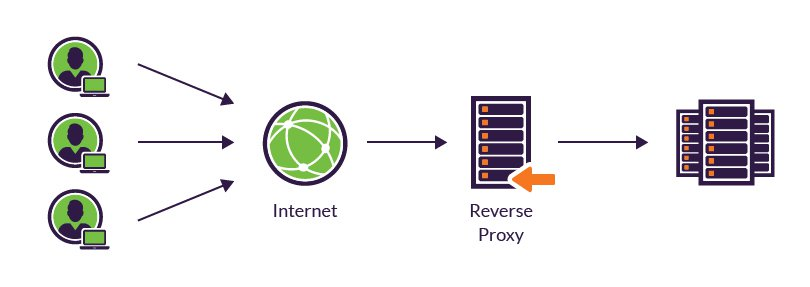
\includegraphics[width=0.5\textwidth]{reverse-proxy-02-1.jpg}
	\caption{Incapsula diagrama reverse proxy}
	\label{fig:reverse-proxy}
\end{figure}

Figura ~\ref{fig:reverse-proxy} ilustreaza modul de functionare al unui reverse proxy in relatie cu serverele aferente si posibili clienti. \\


Conform topului alcatuit de fundatia OWASP cu cele mai mari 10 riscuri ale aplicatiilor in 2017 \cite{owasp}, SQL injection e considerat a fi cea mai mare vulnerabilitate a aplicatiilor web. Acest lucru se datoreaza fatului ca mare parte din aceste aplicatii se bazeaza pe procesearea continutului furnizat de catre utilizatori. Atacurile de tipul SQL injection costau in faptul ca datele furnizate de catre utilizator sunt introduse in interogari SQL, unde acestea sunt tratate ca si cod executabil \cite{classification_and_countermeasures}. Aplicatiile web vulnerabile la sqli injection pot permite unor utilizatori neautorizati sa faca interogari intr-o baza de date asupra unor date la care nu ar avea acces in mod normal. Folosind acest tip de comportament neautorizat, un astfel de utilizator poate sa obtina accesul la informatii sensibile ale clientilor, dar si a administratorilor aplicatiei, precum credentiale sau date personale. Aceasta vulnerabilitate poate sa duca la furt de identitate sau frauda. 

In cazul retelei Tor, aceasta le permite utilizatorilor sa navigheze pe internet anonim. Anonimitatea online este importanta insa in multe cazuri aplicatiile web trebuie sa stie cine se conecteaza la aceasta pentru a le putea determina intentiile. Numele de Tor vine de la "the onion router" care sugereaza modul de operare al retelei. Fiecare participant la retea devine un nod de transfer, iar traficul retelei traverseaza o serie de astfel noduri pana sa ajunga la nodul de iesire ce creaza conexiunea cu destinatia dorita. Pachetele sunt criptate in mai multe "straturi", fiecare nod decriptand un singur strat de unde poate afla doar destinatia nodului urmator. Cand pachetul ajunge la ultimul nod, acesta trimite continutul la destinatie fara sa dezvalui identitatea sursei. Aceasta anonimitate usearaza desfasurarea atacurilor online. Conform datelor din reteaua organizatiei CloudFlare 94\% din traficul provenit din reteaua Tor este alcatuit din request-uri automate de origine malitioasa \cite{tor_trouble}.


%\section{Motivation}
 \section{Motivație}
In piata actuala exista multe sitem de prevenire a intruziunilor ce ofera atat caracteristicile unui reverse proxy, cat si cele de securitate. Aceste caracteristici sunt oferite fie ca si produse individualea, fie ca si produse ce le incorporeaza pe ambele. Cu toate acestea, produsele de acest gen sunt in general scumpe, au o logica mascata de detectarea a posibilelor probleme de securitate si sunt greu de inteles si de configurat de catre utilizator dupa propiile nevoi.

Prin oferirea utilizatorilor posibilitatea de a intelege si modifica modul de functionare a unui astfel de sistem poate rezulta in sisteme mult mai eficiente si rapide, dedicate pentru preferintele si nevoile aplicatiei fiacarui utilizator in parte. Spre exemplu, un utilizator poate sa decida ca nu are nevoie de funcionalitaile de detectie impotriva atacurilor de tip SQL injection pentru o anumita aplicatie, intrucat aceasta nu prezinta vulnerabilitati din acest punct de vedere, nefolosind o arhitectura bazata pe baze de date. In cazul acesta prin eliminarea unui astfel de modul, se elimina si verificarile aferente asupra reques-urilor clientilor, imbutatatind astfel performantele sistemului.

\textit{\thesistitle} ofera un sistem configurabil dupa preferintele utilizatorilor. Utilizatorul poate configura detectia bazata pe analiza request-ului primit de la client, acesta poate sa aleaga  care module sa fie folosite pentru detectie, permitand si eventuala adaugare de noi module(cat timp acestea respecta anumite conditii de structura), meniurile din interfata utilizator fiind generate in mod dinamic in functie de modelele prezente. Utilizator poate, de asemenea sa configureze si lista ip-urilior blocate, permitandu-i-se sastearga din cele existente, respectiva sa aduge unele noi, dupa bunul plac.



%\section{Report's Structure}
 \section{Structura lucrării}
In aceasta sectiune se prezinta structura lucrarii pe capitole si o scurta descriere a continutului acestora:

Primul capitol ~\ref{cap:Introducere}, prezinta o scurta introducere despre proiect, contextul acestuia si motivatia pentru implementarea sistemului propus.

Capitolul~\ref{cap:obiective-specificatii} prezinta obiectivele lucrarii, specificatiile sitemului, motivand deciziile luate in implementarea sistemului, cerintele functionale si nonfunctionale necesare implementarii sistemului.

 Capitolul~\ref{cap:studiu-bibliografic} descrie alte abordari similare ale problemelor tratate de proiectul propus, prin evidentierea asemanarilor si diferentelor dintre acestea si se explica tehnologiile si metodele folosite de proiect.
 
In capitolul~\ref{cap:fund-teoretice} sunt evidentiate si explicate pe scurt aspectele teoretice pe care se bazeaza proiectul.

Capitolul~\ref{cap:analiza-si-proiectare} descrie design-ul proiectului si cuprinde: cerintele sistemului, specificatiile cazurilor de utilizare, arhitectura sistemului, comportamentul sistemului, datele utilizate de sistem, dependintele sistemului si algoritmi esentiali si metodele folosite. Descrierea acestora se realizeaza prin asocierea cu diagramelor aferente.


Capitolul~\ref{cap:implementare} prezinta in amanunt detaliile de implementarea a proiectului. In acest capitol sunt abordate: organizarea codului sursa, descrierea principalelor clase si functionalitati ale proiectului, descrierea  si posibilitatile de desfasurare a executiei programului.

%\chapter{Project's Objectives and Specification}
 \chapter{Obiective și specificații}
\label{cap:obiective-specificatii}

%Acest capitol conține descrierea detaliată a temei de cercetare propriu-zise, formulată exact, cu obiective clare și specificații, pe 2-3 pagini și eventuale figuri explicative. Titlul nu e neapărat impus și, de asemenea, capitolul poate fi inclus ca subcapitol în Capitolul~\ref{cap:Introducere}, dacă se potrivește.
%
%Reprezintă cca. 5--10\% din lucrare.

Acest capitol prezintă obiectivele lucrării, motivând deciziile luate în implementarea sistemului, specificațiile sistemului, cerințele funcționale și nonfunctionale necesare implementării sistemului. 

%\section{Objectives}
 \section{Obiective}
%
%Obiectivele proiectului sunt lucrurile care se dorește a fi realizate, ca urmare a abordării temei lucrării de licență. În general numărul de obiective este proporțional cu timpul de care dispunem. Exemple generice:
%\begin{enumerate}
%  \item Analiza critică a soluțiilor existente pentru problema abordată și identificarea posibile limitări ale acestora.
%  \item Propunerea unor soluții la (o parte) din problemele identificate. 
%  \item Implementarea soluției și validarea ei
%  \item Identificarea unor teme de dezvoltare și cercetare ulterioare
%  \item \dots
%\end{enumerate}
Elaborarea unor măsuri de securitate împotriva anumitor tipuri de atacuri sau dezvoltarea unei logici de filtrare a clienților serviți de către aplicație este posibilă și în partea de implementare a serverului, cea ce ar putea oferi și o eventuală creștere în performanțele aplicației, eliminând astfel posibile interceptări suplimentare și validări ale traficului. Însă o astfel de implementare presupune o arhitectură mult mai complexă pentru partea de server și individual cunoștințe avansate despre securitate, posibilele vulnerabilități la care acesta poate să fie predispus, precum și modalități de combatere ale acestora.  
  
O soluție mult mai simplă la această problemă este folosirea unui modul care să implementeze aceste funcționalități separat. Mare parte din produsele de pe piață, ce îndeplinesc aceste caracteristici sunt destul de scumpe și nu oferă foarte multă libertate din punctul de vedera al configurări securității dorite de către utilizator asupra produsului sau. În cazul IP-urilor blocate, multe aplicații nu oferă libertatea utilizatorilor de a edita listele de referință ale detecțiilor, acestea fiind actualizate automat conform unor date interne, iar eventualele abateri de la aceste reguli se realizează prin adăugarea de excepții. În cea ce privește validarea request-urilor primite de la clienți, mare parte din aceste sisteme nu oferă o protecție configurabilă. Cum sa precizat mai sus, acest tip de sisteme pot să introducă mici întârzieri datorate validărilor suplimentare asupra request-urilor primite de la clienții produsului, însă în unele cazuri anumite validări sunt făcute inutil întrucât produsele respective neputând să prezinte vulnerabilități de acel fel. 

 \textit{\thesistitle}  are obiectivul de a oferi o componentă gratuită cât mai ușor de integrat și de configurat de către utilizator după preferințele produsului sau, care să facilizeze o protecție cât mai eficientă cu suport pentru îmbunătățiri. Sistemul trebuie să fie ușor de instalat și de configurat, oferindu-i utilizatorului o interfață clară, sugestivă și ușor de folosit prin care să interacționeze cu acesta. Detecțiile sistemului trebuie să fie selectabile, utilizator putând alege în momentul pornirii sistemului ce vulnerabilități să fie tratate de acesta. Lista IP-urilor blocate trebuie sa fie ușor de vizualizat și editabila, permițând utilizatorului să își impună cu ușurință propriile reguli asupra modului de funcționare a sistemului. Pentru realizarea detecției împotriva atacurilor de tipul SQL injection se impune prelucrarea unor date reale pentru antrenarea modelului de machine learning. Prin folosirea unor date provenite din atacuri reușite sau tentative de atacuri reale, se poate crea o precizie mult mai bună pentru o clasificarea cât mai precisă a posibilelor atacuri. Sistemul trebuie de asemenea să fie construit modular pentru a permite realizarea de modificări cu ușurință, iar încărcarea detecțiilor realizată dinamic, permițând astfel că adăugarea de noi detecții să fie cât mai simplă. 




%\section{Project Specification}
 \section{Specificații}
\textit{\thesistitle}  trebuie să fie capabil să servească ca și un reverse proxy pentru un server, să blocheze atacurile de tip SQL injection asupra lui și să nu permită conectarea clienților cu IP-uri conținute in lista neagra. 

\textit{\thesistitle}  va procura utilizatorului o interfață grafica prietenoasă, ușor de folosit, prin intermediul căreia, acesta va putea să seteze mediul de rulare al sistemului. Interfața va permite setarea specificațiilor server-ului, adresa și portul pe care acesta acceptă conexiuni, dar și a interfețelor prin intermediul cărora se pot realiza conexiuni la server. 
  
În interfață grafica se vor afișa și eventualele detecții realizate de produs. Într-o fereastră separată utilizatorul trebuie să aibă posibilitatea să vizualizeze toate deciziile sistemului și motivele din spatele deciziilor, permițând astfel acestuia să înțeleagă modul de funcționare, respectiv să raporteze sau să modifice sistemul(în cazurile în care i se oferă această posibilitate) când comportamentul acestuia nu se află în conformitate cu nevoile sau cerințele sale. 

În momentul configurării modului de rulare al sistemului, utilizatorul trebui să aibă și posibilitatea de a impune ce module de securitate să fie folosite de acesta în timpul rulării. Pentru a eficientiza cât mai mult sistemul, utilizatorul poate să aleagă care sunt modulele de interes pentru propria aplicate, evitând astfel validarea unor evenimente ce nu prezintă interes pentru acesta. 

 
În timpul rulării sistemul va asculta pe interfețele setate de către utilizator pentru posibile cereri de conexiuni la server-ul setat. În funcție de modulele alese în momentul porniri, acesta va verifica sau nu adresa clientului validând astfel conexiunea. În cazul în care adresa clientului se află pe lista neagră de adrese, conexiunea acestuia este refuzată, iar aplicația înregistrează această decizie în fereastra de evenimente vizibilă utilizatorului. După realizarea conexiunii la server, fiecare request trimis de clienți către acesta va fi evaluat conform modulelor configurate. Dacă reqest-urile sunt considerate că fiind "curate" acestea sunt trimise mai departe la server. În caz contrar, clientului i se întoarce un cod de eroare, iar reqest-ul nu va mai fi trimis mai departe către server, de asemenea înregistrând evenimentul în fereastra de evenimente vizibilă utilizatorului. 


\begin{figure}[h]
	\centering
	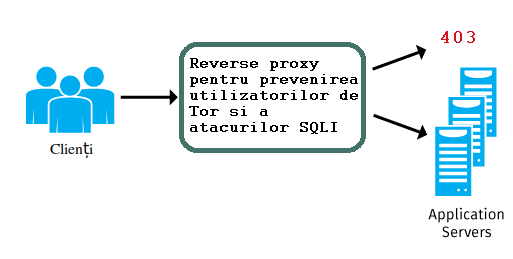
\includegraphics[width=0.6\textwidth]{fff.png}
	\caption{ Cutia neagră a sistemului.}
	\label{fig:black-box}
\end{figure}

Figura ~\ref{fig:black-box} prezintă cutia neagra a sistemului propus. \\

%\subsection{Functional Specification}
 \subsection{Specificații funcționale}

Sistemul trebui să prezinte o interfață grafică ușor de folosit de către utilizator și să fie capabil să redirecționeze traficul interceptat către un anumit server, clasificând și filtrând traficul malițios. Pentru a atinge obiectivele proiectului, următoarele cerințe funcționale trebuie îndeplinite: 
\begin{itemize}
  \item  Să realizeze conexiunea la un server HTTP/HTTPS și să redirecționeze traficul primit către acesta. 
  \item  Să intercepteze traficul venit pe o anumită interfață și port prestabilit. 
  \item  Să prelucreze request-urile primite de la clienți într-un format specific clasificatorului de SQL injection. 
  \item  Să nu redirecționeze reqest-urile clasificate ca și SQL injection. 
  \item  Să blocheze conectarea clienților ce folosesc IP-uri clasificate ca IP-uri de Tor. 
  \item  Să permită utilizatorului să editez și să vizualizeze lista IP-urilor de Tor. 
  \item  Să prezinte în interfața grafică toate intervențiile realizate asupra traficului(blocări de conexiuni sau de request-uri). 
  \item  Să permită utilizatorului să configureze modul de operare al sistemului. 
\end{itemize}


%\subsection{Non-Functional Specification}
 \subsection{Specificații non-funcționale}

Sistemul trebuie, de asemenea, să aibă următoarele caracteristici non-funcționale pentru a realiza obiectivele specificate: 
\begin{itemize}
  \item Să fie ușor de instalat și de folosit pentru orice utilizator, oricât de neexperimentat .
  \item  Să poată intercepta traficul de pe orice/oricâte interfețe disponibile. 
  \item  Să poată rula pe orice sistem de operare Windows cu Python2 instalat. 
  \item  Să aibă o rată de blocare de 100\% a IP-urilor de pe lista neagră, iar 
  în cazul detecției de SQL injection să nu aibă detecții false pozitive mai mari 2-3\% 
  și o acuratețe generală de peste 90\%.
\end{itemize}





%\chapter{Bibliographic Survey}
 \chapter{Studiu bibliografic}
\label{cap:studiu-bibliografic}
%
%Documentarea bibliografică are ca obiectiv fixarea referențialului în care se situează tema, prezentarea susrselor bibliografice utilizate și a cercetărilor similare și raportarea abordării din lucrare la acestea.
%
%Referințele bibliografice se vor face pentru fiecare carte, articol sau material folosit pentru elaborarea lucrării de licență. 
%
%Reprezintă cca. 10--15\% din lucrare.
În acest capitol sunt prezentate alte abordări similare ale problemelor tratate de proiectul propus, prin evidențierea asemănărilor și diferențelor dintre acestea și se explică tehnologiile și metodele folosite de proiect. 

%\section{Related Work}
 \section{Abordări similare}

%Comparați abordarea  motivand deciziile luate in implementarea sistemului, cu cele ale altor soluții: ce e asemănător, ce e diferit (și, de preferat, mai bun). 
%
%Citarea referințelor se face ca în exemplele \ref{subsec:s10} din Bibliografie. 
%Vezi citările următoare.
%
%În articolul [] autorul descrie configurația tehnică a unei "honeynet" și prezintă câteva atacuri de actualitate asupra honeynet, precum și o serie de recomandări pentru securizarea sistemelor conectate la rețele de calculatoare.

% În capitolul 4 al [], referitor la valoare honeypots, Spitzner prezintă avantajele și dezavantajele acestora.

%În articolul on-line [] găsim detalii interesante despre \dots.


%\section{Technologies and Methods}

Precum Richard Bassett, Cesar Urrutia si 	 Nick Ierace sustin in articolul \textbf{Intrusion prevention systems} \cite{ips}  "sistemele de prevenire a intruziunilor sunt o componentă importanata a sistemelor de protecție IT, iar fără această tehnologie, datele noastre și rețelele ar fi mult mai predispuse activităților malițioase". 

În general tentativele de expluatare a vulnerabilităților unei aplicații vin sub formă de input către o aplicația țintă. Acest input fiind generat de către un atacator ce intenționează o controleze sau să îi întrerupă activitatea. În cazul unui atac reușit, un astfel de atacator poate să dezactiveze temporar aplicația (atacuri de tipul denial of service) sau poate accesa, altera sau executa date/cod în interiorul aplicației. Un sistem de prevenire a intruziunilor are rolul de a examina traficul destinat unei aplicații și de intercepta și bloca astfel de tentative  \cite{what_is_ips}.

Un sistem de prevenire a intruziunilor este de regulă folosit alături de un sistem firewall respectiv alături de un sistem de detectare a intruziunilor. Deși au scopuri asemănătoarea, aceste sisteme au funcționalități diferite și rezolvă diferite probleme de securitate. Un sistem de prevenție a instrucțiunilor este cel mai bine comaprat cu sistemele de tip firewall. Un sistem firewall tipic este constituit dintr-o serie de reguli ce permit traficului să treacă. Aceste regului sunt sub forma "dacă traficul îndeplinește anumite condiții poate trece", însă dacă nu există nici o regulă care să potrivească anumite pachete, acestea sunt blocate. Asemeni sistemelor firewall, sistemele de prevenire a intruziunilor prezintă un set de regului de filtrare a pachetelor, reqest-urilor  sau a clienților, însă aceste regului sunt de regulă reguli de blocare. Astfel, dacă un anumit pachet nu potrivește nici o regulă sistemul de prevenire a intruziunilor îl lasă să treacă  \cite{ips_ids}.

Spre deosebire de sistemele de tip firewall sau cele de prevenire a intruziunilor, care oferă control utilizatorului asupra traficului ce trece prin rețea, sistemele de detecție a intruziunilor permite acestuia să vizualizeze evenimentele din rețea. Precum și Joel Snyder susține în articolul  \textbf{Do you need an IDS or IPS, or both?} \cite{ips_ids}  sistemele  de detecție a intruziunilor oferă unui utilizator facilități asemănătoare unui analizator de pachete  \cite{net_an},  însă din perspectiva de securitate a rețelei. Aceste informații furnizate de către sistem îi permit utilizatorului să decopere:  
 
\begin{itemize}
	\item  Încălcări ale politicilor de securitate, precum utilizatori sau siteme ce desfășoară activități ce încalcă politicile prestabilite. 
	\item  Posibile sisteme infectate ce folosesc rețeaua pentru a se răspândi sau să atace alte sisteme. 
	\item  Scurgeri de informație cauzate de infectarea unor sisteme cu malwarei sau de utilizatori rău intenționați. 
	\item  Erori de configurare în sisteme sau aplicații cu setări de securitate incorecte sau configurări proaste ce consumă prea multă bandă de rețea. 
	\item  Detectarea unor clienți sau servere ce accesează sau sunt accesate în mod neautorizat, respectiv aplicații malițioase ce fac asta. 
\end{itemize}
\begin{figure}[h]
	\centering
	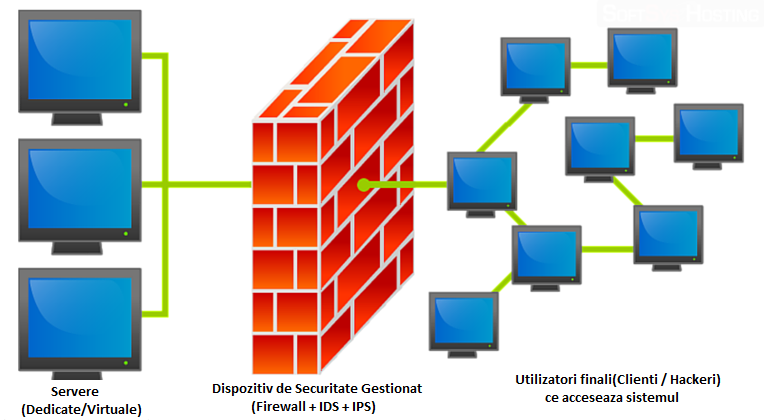
\includegraphics[width=0.6\textwidth]{ips.png}
	\caption{ Administrarea securității unei aplicații }
	\label{fig:ips-example}
\end{figure}

Figura ~\ref{fig:ips-example}  prezintă administrarea securității unei aplicații folosind combinația dintre cele trei sisteme.  \\

În comparație cu sistemele de detecție a intruziunilor care sunt sisteme pasive și scanează rețeaua fără să interferezu cu traficul, sistemele de prevenire a intruziunilor sunt plasate între server și cilenti, alterând în mod automat traficul în cazul în care acesta declanșează una din regulile prezente în sistem. Precum sunt prezentate și în articolul  \textbf{What is an intrusion prevention system?} \cite{what_is_ips},  printre funcționalitățile unui sistem de prevenire a intruziunilor se număra:
\begin{itemize}
	\item  Notificarea unui administrator de rețea în cazul în care una sau mai multe reguli sunt declanșate. 
	\item  Oprirea pachetelor considerate malițioase pentru rețea.
	\item  Blocarea unor utilizatori prin excluderea adreselor IP ale acestora. 
	\item  Resetarea unor conexiuni. 
\end{itemize}

În cea ce privește funcționalitățile oferite de un sistem de prevnire a intruziunilor, acestea sunt specifice tipului sistemului. Conform autorului articoluiui \textbf{Intrusion Prevention System (IPS): Definition \& Types} \cite{ips_types}, Beth Hendricks,  există patru tipuri primare de astfel de sisteme: 
\begin{itemize}
	\item Network-based: Protejeaza intraga rețea.
	\item Wireless: Protejeaza doar rețeaua wireless.
	\item Network behavior: Examineaza traficul din rețea.
	\item Host-based: Software cu scopul de a proteja un singur calculator.
\end{itemize}

Sistemele de tipul Network-based(reprezentand și categoria in care se incadreaza  \textit{\thesistitle})  presupun implementarea unor senzori în rețea carea capturează și analizează traficul ce trece prin acesta. Acești senzori sunt plasați în puncte cheie a rețelei pentru a putea captura în timp real traficul, iar în cazul interceptării unor activități malițioase să poată interveni imediat, fără să scadă performanța rețelei. Aceste siteme oferă protecție rețelei indiferent de dimensiunilie sau creșterea acesteia, adăugarea de noi device-uri fiind posibilă fără să necesite adăugarea de noi senziori. Adăugarea de noi senzori fiind nevoită doar în cazul în care traficul rețelei depășește capacitatea de procesarea a senzorilor curenți, infulentand astfel performanțele rețelei \cite{impl}.

În funcție de nevoi, un sistem de prevenire a intruziunilor poate să ofere diferite opțiuni de protecție pentru diferite părți ale rețelei. Unele sunt capabile să oprească traficul malițios sau să limiteze lățimea de bandă către anumite părți ale rețelei. Conform \cite{ips_sec_types} aceste siteme pot oferi protecți împotriva următoarelor tipuri de atacuri: 
\begin{itemize}
	\item \textbf{ICMP Storms:}  un volum mare de ecouri ICMP pot să indice activități malițioase precum cineva ce scanează rețeaua. 
	\item \textbf{Ping to Death:}  un utilizator poate să modifice comandă de ping, astfel încât să trimită un număr mare de pachete de dimensiune mare către o destinație țintă pentru a o scoate din uz. 
	\item \textbf{SSL Evasion:}  unele atacuri se pot folosi de criptarea SSL pentru a evita dispozitivele de securitate, întrucât în general acestea nu sunt decriptate. 
	\item \textbf{IP Fragmentation:}  constă în expluatarea faptului că pachetele sunt descompuse în fragmente pentru a staisface cerințele de dimensiune a rețelelor traversate, inundând o destinație țintă cu fragmente false pentru a îi consuma resursele.  
	\item \textbf{SMTP mass mailing attacks:}  un sistem infectat poate să se folosească de email-ul utilizatorului pentru a se răspândi, rezultând într-un trafic mare destinat serverului de mail. 
	\item \textbf{DoS/DDoS attacks:} cu scopul de a face o resursa indisponibilă utilizatorilor, este realizată prin inundarea sistemului țintă cu un număr mare request-uri de la unul sau mai multe(în cazul Dos distribuit-DDoS) siteme malițioase. 
	\item \textbf{SYN Flood attacks:}  atacatorul trimite un număr mare de pachete de initiare a unei conexiuni fără să mai răspundă ulterior, epuizând astfel resursele de memorie. 
	\item \textbf{Http obfuscation:}  pentru a evita să fie detectate de anumite siteme de protecție, unele atacuri folosesc tehnici de ofuscare a request-urilor HTTP. 
	\item \textbf{Port Scanning:}  este folosit pentru descoperi ce porturi sunt deschise pe un sistem, ulterior permițându-i atacatorului să știe ce vulnerabilități ar putea prezneta sistemul. 
	\item \textbf{ARP Spoofing:}  un atacator trimite în rețea pachete false de ARP legându-și propria adresă MAC de adresa IP a unui alt sistem. Ca urmare, atacatorul va primi pachete destinate sistemului cu adresa IP folosită în pachetul de ARP. 
	\item \textbf{CGI Attacks:}  un atacator poate să trimită request-uri malițioase, determinând destinația să trateze request-ul primit ca și cod executabil, oferindu-i atacatorului acces pe sistem. 
	\item \textbf{Buffer Overflow attacks:}  presupune ca atacatorul să depășească limitele unui buffer de lungime fixă, excesul de date ajungând să suprascrie zone adiacente de memorie rezultând în căderea sistemului sau dându-i atacatorului oportunitatea să ruleze cod propriu. 
	\item \textbf{OS Fingerprinting attacks:}  presupune ca atacatorul să descopere ce sistem de operare rulează pe un sistem și folosindu-se de această informație să expluateze vulnerabilități specifice acelui sistem de operare. 
\end{itemize}

Sistemul propus, \textit{\thesistitle}  implementează un sistem de prevenire a intruziunilor folosindu-se de un reverse proxy pentru a intercepta tot traficul care intră și iese din rețea (reprezentând senzorii ce au rol de a captura și analiza traficul) și oferind protecție împotriva a două categorii de atacuri: orpirea de URL-urilor malițioase destinate unei aplicații(protecție împotriva SQL injection) și blocarea adreselor IP cunoscute ca fiind folosite de utilizatori rău intenționați(protecție împotriva adreselor IP ale rețelei Tor). 

Pentru prevenirea atacurilor de SQL injection, se folosește o metodă asemănătoare celei propuse de Eun Hong Cheon, Zhongyue Huang și Yon Sik Lee în lucrarea  \textbf{Preventing SQL Injection Attack Based on Machine Learning} \cite{sqli_how}. Pentru clasifiacrea request-urilor HTTP în SQL injection sau curate, se folosește un sistem bazat pe machine learning. Acest sistem este antrnat anterior cu date reale, ca și trăsături fundamentale în clasificare, folosindu-se cuvintele cheie și simbolurile specifice limbajului SQL(spre exemplu: SELECT, ADD, DELETE, ", ' etc.). 

\begin{figure}[h]
\centering
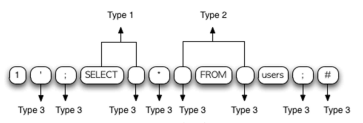
\includegraphics[width=0.6\textwidth]{sqli.png}
\caption{ Tipuri de trăsături ale limbajului SQL }
\label{fig:sql-features}
\end{figure}

Figura ~\ref{fig:sql-features}  prezintă tipurile de trăsături luate în considerare în lucrarea \textbf{Preventing SQL Injection Attack Based on Machine Learning} în raport cu simbolurile sau cuvintele cheie folosite.  


 O altă abordare pentru prevenirea atacurilor SQLI este propusă de Fredrik Valeur, Darren Mutz și Giovanni Vigna în lucrarea \textbf{A Learning-Based Approach to the Detection of SQL Attacks} \cite{sqli_how2}. În această lucrarea se prezintă folosirea unui sistem bazat pe detecția de anomalii pentru detectarea atacurilor ce expluateaza o aplicație pentru a îi compromite baza de date. Asemeni abordării bazate pe machine learning, acest sistem presupune o fază anterioară de antrenare în care se învață comportamentul normal al utilizatorilor, alcătuind astfel niște profile specifice. Astfel în faza de detecție, comportamentul ce nu coincide cu profilele alcătuite în faza de antrenate, este considerat malițios. 

Pentru prevenirea utilizatorilor de Tor, în general lista de IP-uri este alcătuită din toate IP-urile care au utilizat rețeaua într-un anumit interval de timp, aceasta fiind actualizată periodic. O astfel de abordare este folosită și în cazul marelui firewall al Chinei  \cite{china_tor}  care indentifică nodurile la prima accesare a rețelei de Tor. Însă precum precum se evidențiază și în articolul  \textbf{Characterizing the Nature and Dynamics of Tor Exit Blocking} \cite{tor_1} o astfel de abordare nu este cinstită față de unii utilizatori de Tor, întrucât reputația acestora este împărțită între toți utilizatorii. Astfel un nod care este utilizat doar pentru câteva minute sau ore(probabil din motive de curiozitate) poate să ajungă să fie blocat, fiind tratat asemeni cu un nod ce functionaza de câteva zile. O astfel de discriminare a încercat să fie evitată prin implementarea aleasă a sistemului propus. Pentru realizarea listei de IP-uri blocate se folosește un algoritm ce stabilește o limită de timp minima de funcționare pentru un anumit nod în intervalul a 30 de zile. 


 \section{Tehnici/Tehnologii/Surse folosite}

Pentru realizarea sistemului propus s-au folosit două limbaje de programare: Pyhton2/3(pentru partea de back end) și C\#(pentru partea de front end). În partea de back end a proiectului se realizează implementarea unui reverse proxy pentru a intercepta traficul uneia sau mai multor interfețe, un modul pentru clasificarea request-urilor împotriva atacurilor SQL injection și un modul pentru generarea listei negre de IP-uri ce utilizează frecvent rețeaua Tor. Toate aceste componente sunt realizate prin utilizarea de librării open-source pentru a ușura și eficientiza munca precum:  twisted \cite{twisted}, beautiful soup \cite{btf_soup}, libsvm \cite{libsvm}.

Motivul utilizării atât limbajului Python3 cât și Python2 este datorat diferențelor de module și librării open-source disponibile pentru cele două limbaje dar și a faptului că suportul pentru Python2 se închei în anul 2020. Conform documentațiilor oficiale  \cite{python3_doc} și \cite{python2_doc}, dar și articolului \textit{Python 2 to python 3: why, and how hard can it be?} de Tim Grey \cite{why_python3},  între cele două versiuni nu sunt modificări majore, însă în anumite cazuri pot există librării care să ofere doar suport pentru una dintre aceastea. 

În realizarea modulului pentru clasificarea request-urilor împotriva atacurilor SQL injection să folosit o colecție de date reale atât de atacuri cât și de trafic curat. Pentru uniformizarea acestor date și pentru a trata tentativele de păcălire a clafisicatorului prin codarea unor caractere în valoarea lor în cod hexadecimal (exemplu 'https://www.google.ro /search?q=a' echivalent cu 'https://www.google.ro/search?q=\%61') datele au fost preprocesate și transformate în întregime în coduri hexadecimale  \cite{ascii}.  În procesarea datelor, pentru indetificarea trăsăturilor relevant, s-au indentificat caracterele specifice limbajului \cite{char_sql} si cuvintele cheie rezervare \cite{key_sql}. Ulterior, pentru antrenarea modelului de support vector machine și pentru clasificarea noilor request-uri s-a folosit software-ul open-source libsvm \cite{libsvm_class}. 

\begin{figure}[h]
	\centering
	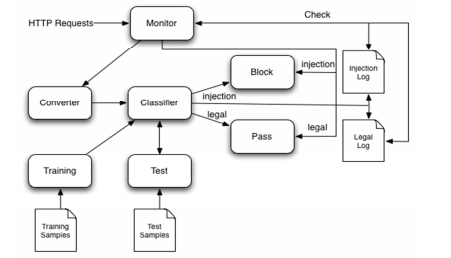
\includegraphics[width=0.6\textwidth]{sql_arh.png}
	\caption{Arhitectura unui sistem de clasificare a request-urilor HTTP}
	\label{fig:sql-arh}
\end{figure}

Figura ~\ref{fig:sql-arh}  prezintă arhitectura unui sistem de clasificare a request-urilor HTTP de un sistem bazat pe machine learning. Structura este prezentată în lucrarea prezentată și anterior  \textbf{Preventing SQL Injection Attack Based on Machine Learning} \cite{sqli_how}.  Acesta structură a reprezentat un model de pornire în realizarea modulului de prevenire a atacurilor SQL injection, implementarea modulului încercând să aducă îmbunătățiri de performanță prin modificarea algoritmului folosit pentru antrenarea modelului de support vector machine, dar și prin filtrarea trăsăturilor propus în lucrare în conformitate cu raportul dintre obișnuința de apariție a acestora atât în request-urile ce intenționează să execute un atac cât și în cele curate. 

Pentru blocarea IP-urilor utilizate de reteua Tor s-a folosit un script scris în Python3. Programul interoghează periodic(din 6 în 6 ore) informațiile oferite de \textit{Tor Network Status} \cite{tot_status} indentificand astfel nodurile cu un "Uptime" mai mare de 7 zile în parcursul unei luni. Blocarea IP-urilor se realizează prin compararea cu o astfel de listă generată lunar. 

Componenta ce încorporează toate modulele de protecție, este cea de reverse proxy. Aici este monitorizat tot traficul ce vine de pe o anumită interfață(una sau mai multe, în funcție de configurația utilizatorului) și este trecut prin toate modulele disponibile pentru a verifica condițiile de securitate. Pentru testarea dacă o adresă IP este utilizată frecvent de rețeaua Tor, în momentul în care un client dorește să realizaze o conexiune la server-ul protejat de sistem, adresa IP a acestuia este verificată să nu se afle pe lista IP-urilor blocate. Pentru actualitate, lista adreselor IP blocate este actualizată periodic cu adresele IP utilizate frecvent de rețeaua Tor în ultima luna. Modulul de prevenire a atacurilor SQL injection este integrat tot în componenta de reverse proxy, însă evaluarea request-urilor este făcută după realizarea conexiunii între client și server. Request-urile primite de către server sunt tratate asemănător celor folosite pentru antrenarea modulului de support vector machine, însă pentru clasificarea acestora este folosit modulul antrenat în fază inițială și software-ul de prezicere oferit tot de libsvm \cite{libsvm}.
	
	

	






% \chapter{Theoretical Backgound}
\chapter{Fundamente teoretice}
\label{cap:fund-teoretice}


In acest capitol sunt evidentiate si explicate pe scurt aspectele teoretice pe care se bazeaza proiectul.

%
%Aici se descriu pe scurt aspecte teoretice pe care se bazează lucrarea. Conținutul acestui capitol trebuie gândit pentru un citor care nu e specializat pe domeniul temei și nu cunoaște chestiunile de bază despre subiect. Pentru un cititor specializat, capitolul poate să stabilească un limbaj comun, relativ la termenii care pot fi interpretați diferit. 
%
%Acest capitol nu trebuie gândit și scris nici ca un copy-paste din alte surse, nici ca zona de reglaj a numărului de pagini ale lucrării. Deși va conține chestiuni pe care le-ați studiat și voi și pe care v-ați bazat, el trebuie să fie o compilare a surselor folosite, care să aibă sens și relevanță pentru lucrarea voastră. Trebuie să fie o descriere coerentă și logică a unor aspecte care ușurează sau fac posibilă înțelegerea părților următoare ale lucrării. Nu trebuie intrat insă prea mult în detalii, ci spuse doar chestiunile esențiale. 
%
%Dacă preluați text, figuri, tabela etc. din sursele de documentare, acestea din urmă trebuie indicate explicit. 
%
%Reprezintă cca. 10--15\% din lucrare.
\section{Reverse proxy}

Un reverse proxy este un server intermediar care trimite mai departe request-urile pentru continut de la mai multi clienti nedefiniti catre unul sau mai multe servere. Un reverse proxy este un tip de proxy care in mod normal este situat in spatele unui firewall intr-o retea interna si redirectioneaza traficul clientilor catre serverele asociate. Acesta introduce un nivel in plus de abstractizare si control, asigurand controlul fluxului de trafic \cite{rev_proxy_server}.

\begin{figure}[h]
	\centering
	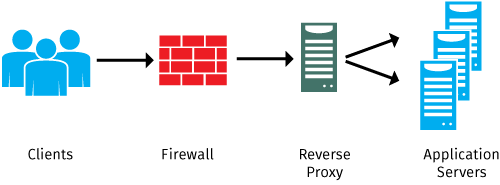
\includegraphics[width=0.6\textwidth]{rev-proxy.png}
	\caption{Folosirea unui reverse proxy in arhitectura unei aplicatii.}
	\label{fig:rev-proxy}
\end{figure}

Figura ~\ref{fig:rev-proxy} prezinta modalitatea de integrare a unui reverse proxy in implementarea arhitecturii de back end a unei aplicatii. \\

Cele mai obisnuite caracteristici ce pot fi oferite de utilizarea unui reverse proxy sunt:
\begin{itemize}
	\item Load balancing - un reverse proxy poate sa distribuie request-urile primite de la clienti, astfel incat nici un server sa nu fie coplesit ce reqesturi. In cazul in care un server este supraincarcat cu reqest-uri sau este cazut, acesta poate sa redirectioneze traficul carea alte servere functionale.
	\item Web acceleration - un reverse proxy poate sa realizeze compresia datelor sau sa memoreze in memoria cache continut ce este frecvent accesat sau poate sa realizeze operatiile de criptare SSL executate in mod normal de server, imbunatatind astfel in mod considerabil viteza de comunicare dintra client si serverul destinatie.
	\item Securitate si anonimitate - prin interceptarea request-urilor primite de catre server, acesta asigura anonimitatea serverului actionand ca un nivel extra de securitate. De asemenea se asigura ca mai multe servere pot fi accesate prin intermediul unui punct comun, indiferent de structura retelei interne.
\end{itemize}



\section{Support vector machine}

Algoritmul de machine learning, support vector machine reprezinta un model obtinut prin folosire a diversi algoritmi pentru antrenarea acestuia, folosit pentru a clasifica date. Acest model intra in categoria de invatare supravegheata('supervised learning'), intrucat pentru obtinerea lui se foloseste un set de date ca si exemplu, date pe care modelul le va folosi ca referinta pentru clasificarea noilor evenimente.

Realizarea unui astfel de model se obtine in urma executarii unui proces elaborat ce implica mai multi pasi:
\begin{itemize}
	\item  Primul pas reprezinta indentificarea datelor relevante in cea ce priveste problema tratata(setul de antrenare). In conformitate cu scopul clasificarii unor evenimente/date in doua(sau mai multe) categorii, initial trebuie indentificate o serie de astfel de evenimente si categorizate de catre utilizator in evenimente ce sigur apartin fiecarei dintre categoriile tinta.
	\item Dupa  obtinerea datelor de antrenare, trebuie indentificate toate trasaturile relevante din aceste date, trasaturi care sa fie cat se poate de specifice fiecarei categorii in parte. Fiind recomandata evitarea trasaturilor ce sunt prezente in mare parte din date sub aceasi forma (ex:caracterul '=' sau'?' intr-un URI folosit pentru clasificarea atacurilor SQL injection), indiferent de categoria din care acestea fac parte.
	\item Dupa obtinerea trasaturilor specifice datelor de antrenare, se realizeaza antrenarea modelului folosind un algoritm specific. In cazul proiectului propus s-a folsoit algoritmul gata implementat, furnizat de biblioteca open source LIBSVM \cite{libsvm}. Pentru obtinerea modelului datele de antrenare au fost procesate folosind un kernel gausian. Un kernel gausian reprezinta modul in care modelul proceseaza datele de antrenare astfel incat clasificarea noilor date sa fie realizata prin calcularea similaritatilor dintre acestea si cele de antrenare. In calcularea similaritatii dintre aceste doua tipuri de date, un parametru foare important este sigma. Acest parametru este ales pentru intrg setul de date, iar valoarea lui este diret proportionala cu gradul de similaritate pe care algoritmul il va asocia la doua evenimente/date diferite.
\end{itemize}



\begin{figure}[h]
	\centering
	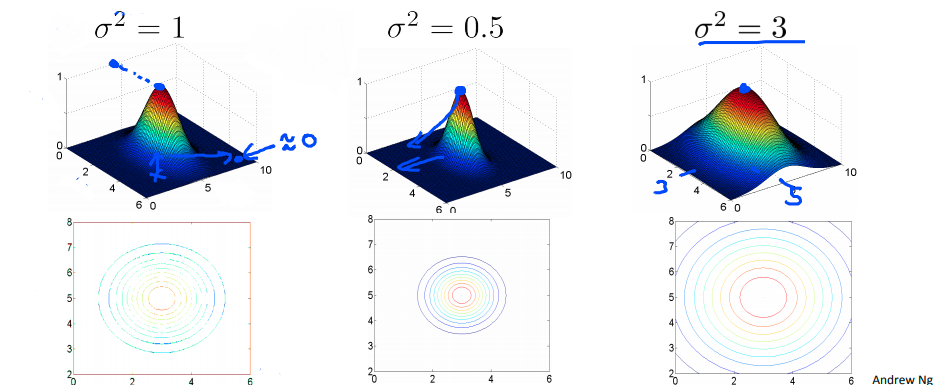
\includegraphics[width=0.8\textwidth]{svm-andrew.png}
	\caption{Influentele aduse algoritmului de modifiacrea parametrului sigma in algoritmul de antrenare.}
	\label{fig:rev-proxy}
\end{figure}

Figura ~\ref{fig:rev-proxy} prezinta cum inflenteaza clasificarea unui nou eveniment valoarea parametrului sigma din formula algoritmului de support vector machine. Figura ~\ref{fig:rev-proxy} a fost preluata din slide-urile cursului de machine leraning sustinut de Andrew Ng \cite{andrew_ng} \\


\section{SQL injection}

Atacurile de tipul SQL injection sunt realizate prin injectarea de cod executabil intr-o baza de date.

Procesul de interactionare cu o baza de date presupene realizarea de interogari asupra acesteia. In formularea acestor interogari, utilizatorul trebuie sa prezinte interpretorului, sub forma de siruri de caractere, numele tabelelor interogate sau valorile unor capuri specifice din acestea. Aceste siruri de caractere sunt delimitate folosind caracterul " sau '. Atacurile de tipul SQL injection expluateaza folosirea acestor delimitatori de siruri de caratere, trimitand siruri de caractere eronate intentionat catre baza de date. Un utilizator rau intentionat poate sa furnizeze astfel de siruri de caractere catre o baze de date prin intermediul oricarui procesator de continut disponibil unui client al unei aplicatii ce comunica cu o baza de date. Aceste siruri de caractere delimiteaza prematur valoarea care este folosita in interogare, introducand dupa aceasta o serie de caractere pe care interpretorul le va trata ca si cod executabil, oferindui astfel utilizatorului sa execute operatiuni asupra bazei de date la care nu ar avea accesul in mod normal. Aceste operatiuni pot sa reprezinte alterarea bazei de date sau obtinerea de date confidentiale. \\



\begin{figure}[h]
	\centering
	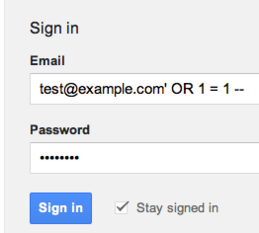
\includegraphics[width=0.4\textwidth]{259px-Sql_Injection_Login.png}
	\caption{Exemplu de atac realizat prin SQL injection.}
	\label{fig:sqli-example}
\end{figure}

Figura ~\ref{fig:sqli-example} prezinta o tenatativa de atac prin SQL injection in care in campul de validare a email-ului se incearca injectarea de cod ce va fi executat in interogarea de validare a credentialelor. Prin prezenta caracterului ' se escapeaza tot textul urmat dupa acesta ca fiind cod si nu un string ce face parte din campul de email. Operatia logica "OR 1=1" va determina interpretorul sa returneze adevarat(valid) pentru orice adresa de email introdusa introdusa inaintea caractrului '. \\


\section{Adresele IP ale retelei Tor}
Reteaua Tor reprezinta un softrware gratis de anonimizare a traficului pe internet. Numele este de fapt un actonim pentru "The Onion Router"(router-ul ceapa) care sugereaza modul de functionarea al acestuia, ficare nod din retea adugand un strat extra de securitate celor precedente. Modul de functionare al retelei se bazeaza pe rutarea traficului prin cat mai multe noduri pentru a anonimiza si a face cat mai greu de urmarit traficul unei anumite persoane. Aceste noduri prin care traficul este directionat sunt sustinute gratis de catre voluntari/utilizatori de Tor din intreaga lume.

Pentru criptarea traficului reteaua Tor foloseste criptarea la nivelul aplicatiei in cea ce priveste sructura retelelor de calculatoare(modelul OSI sau TCP/IP). Datele trasmise sunt criptate, incluzand destinatia, cu exceptia nodului urmator, astfel creandu-se structura de "ceapa" asupra unui pachet. Selectia nodurilor prin care se face rutarea pachetelor este aleasa random. Fiecare pachet decripteaza un "strat", afand nodul urmator pentru pachetul respectiv, nodul final decriptand datele initiale si realizand trasmisia catre destinatie, fara sa ii comunice sursa pachetului. Intrucat in comunicarea pachetelor, pe parcursul rutelor parcurse, se cunoaste in permanenta doar nodul urmator, acest lucru impiedica monitorizarea traficului intre sursa si destinatie.


Cu toate ca reteua tor ofera anonimitate de partea clientului, acest lucru nu se realizeaza si faca de ea. Reteaua nu se ascunde fata de serviciile acesate prin intermediul ei. Astfel un site anume poate sa detecteze daca un anumit client il acceseaza folosind reteaua Tor sau nu.

Intrucat reteaua Tor nu isi ascunde adresele ip folosite de catre aceasta, indentificarea lor si procurarea de date despe acestea este destul de usoara. In proiectul propus s-a folosit un serviciu care furnizeaza gratui astfel de date \cite{tot_status}(adresa ip, uptime etc.) si s-au folosit algoritmi propri pentru procesarea acestor date, eliminand astfel necorectitudinea dintre utilizatorii retelei.

\begin{figure}[h]
	\centering
	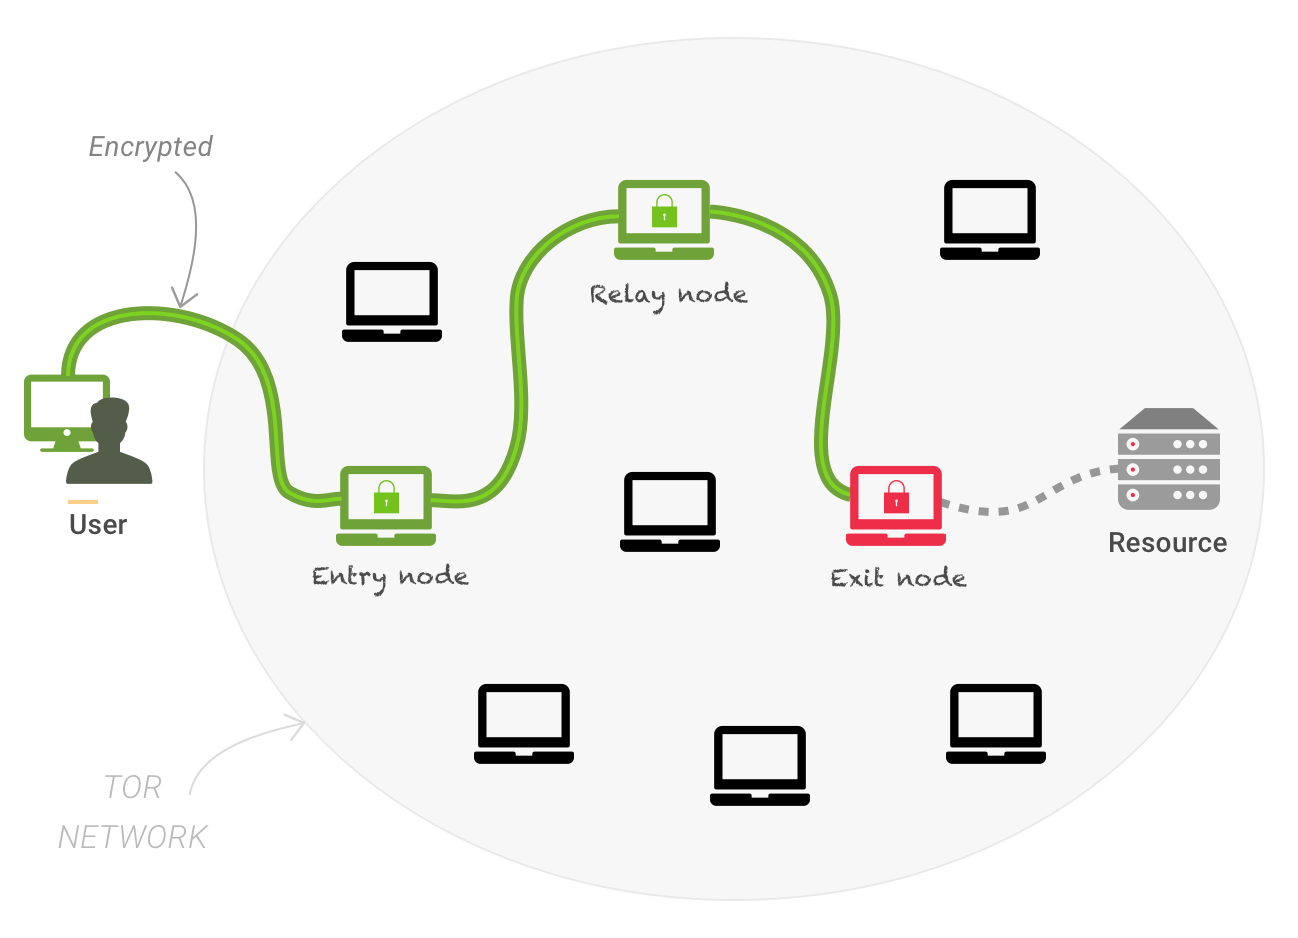
\includegraphics[width=0.6\textwidth]{can-you-hide-on-Tor-Network.png}
	\caption{Exemplu de trafic realizat prin reteaua Tor.}
	\label{fig:tor-example}
\end{figure}

Figura ~\ref{fig:tor-example} prezinta principalele elemente folosite la rutarea treficului de la client la destinatie prin intermediul retelei Tor. \\


\section{Sistem de prevenire a intruziunilor}
Conform scurtei descrieri prezentate in capitolul anterior, un sistem de prevenire a intruziunilor are rolul de a filtra traficul dintre clientii unui server si serverul propiu zis. 

Acest sistem functioneaza liniar, adica este plasat direct intre server si clienti acestuia. In cazul proiectului propus, componenta de baza pentru interceptarea traficului este realizata prin implementarea unui reverse proxy, oferind astfel caracteristica de interceptare si decriptare a traficului, ce permite analiza acestuia, dar si avantajele specifice utilizarii unui reverse proxy.

Pentru filtrarea traficului, un sistem de prevenire a intruziunilor implementeaza anumiti senzori care au rolul sa inspecteze tot traficul ce trece prin sistem, realizand aceasta inspectie in timp real. Datorita acestei verificari, orice pachet considerat malitios este oprit din a ajunge la serverul destinatie. In proiectul propus, implementarea acestor senzori este realizata in doua moduri. In cazul validarii adreselor ip impotriva utilizatorilor de Tor se folosete o lista de ip-uri ce contine adrese frecvent utilizate de reteaua Tor. In interiorul reverse proxy-ului, in momentul crearii unei noi conexiuni, acesta verfica ca adresa ip ce solicita conectarea la server sa nu fie continuta de lista mentionata. In cazul detectiei impotriva atacurilor de SQL injection, senzorul este implementat prin utilizeaza un model de support vector machine. In interiorul reverse proxy-ului in momentul interceptarii unui request venit din exterior catre reteaua interna, acesta verifa daca reqestul poate fi clasificat ca si tentativa de atac, in caz afirmativ blocand trecerea acestuia mai departe catre server.
\begin{figure}[h]
	\centering
	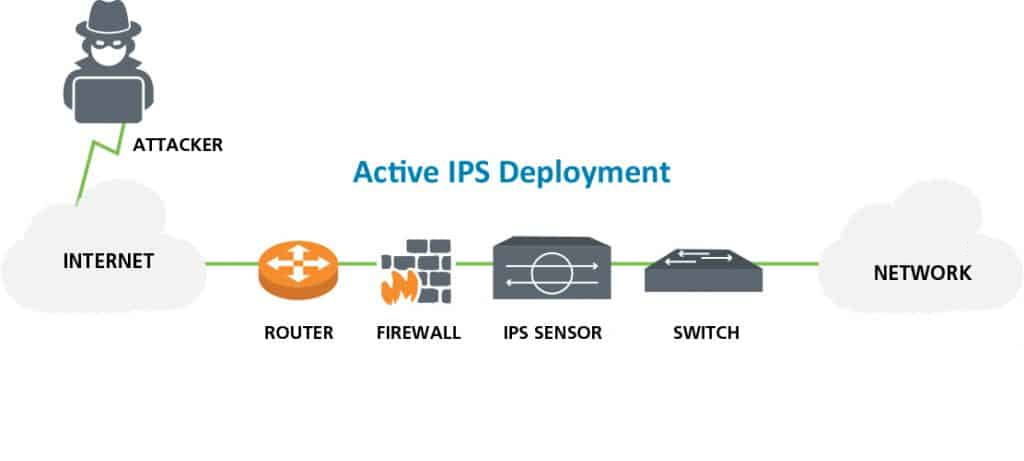
\includegraphics[width=0.6\textwidth]{IPS.png}
	\caption{Integrarea unui sistem de prevenire a intruziunilor intr-o retea.}
	\label{fig:ips-2nd-example}
\end{figure}

Figura ~\ref{fig:ips-2nd-example} prezinta arhitectura unei retele interne ce integreaza un sistem de prevenire a intruziunilor pentru protejarea acesteia. \\
Un sistem de prevenire a intruziunilor poate sa efectueze oricare din urmatoarele actiuni in momentul detectarii unui eveniment malitios \cite{ips_fire}:
\begin{itemize}
%	Terminates the TCP session that is being exploited by an outsider for the attack. It blocks the offending user account or source IP address that attempts to access the target host, application, or other resources unethically.
	\item Sa intrerupa sesiunea dintre client si server, in cazul in care clientul desfasoara sau incearca sa desfasoare activitati malitioase in reteaua protejata de sistem. Acest lucru se poate realiza prin blocarea anumitor credentiale asociate cu utilizatorul respectiv sau prin blocarea adresei ip a acestuia.
	\item In conditiile in care un sistem de prevenire a intruziunilor detecteaza clasifica o activitate ca fiind malitioasa, acesta poate sa ia masuri automat pentru a preveni un astfel de atac pe viitor(ex: in momentul detectarii unei tentative de atac prin SQL injection, sistemul de prevenire a intruziunilor poate sa blocheze in mod automat adresa ip a utilizatorului ce inceraca sa faca atacul, nepermitandu-i acestuia sa se mai conecteze la serverul destinatie pentru un anumit interval de timp sau pana la interventia unui administrator).
	\item O alata abordare posibila in momentul declansarii unui eveniment malitios este alterarea traficului astfel incat sa elimine continutul malitios din acesta. Pentru realizarea acestui lucru, un sistem de prevenire a intruziunilor poate sa stearga atasamente infectate din interiorul unui mail, sa altereze continutul uni pachet sau sa omita trasmiterea mai departe a unor pachete.
	
\end{itemize}


%\chapter{Analysis and Design}
\chapter{Analiză și proiectare}
\label{cap:analiza-si-proiectare}

In acest capitol este descris design-ul proiectului si cuprinde: cerintele sistemului, specificatiile cazurilor de utilizare, arhitectura sistemului, comportamentul sistemului, datele utilizate de sistem, dependintele sistemului si algoritmi esentiali si metodele folosite. Descrierea acestora se realizeaza prin asocierea cu diagramelor aferente.

\section{Cerintele sistemului}

Sistemul propus \textit{\thesistitle} reprezinta un software gratis care ofera clientului atat caracteristici specificie unui reverse proxy, cat si modalitati de protectie asemeni unui sistem de prevenire a intruziunilor.
Sistemul este usor de instalat si de utilizat, chiar si de catre utilizatorii neexperimentati, oferindu-le acestora o interfata clara si sugestiva, ce mascheaza logica complicata din spate. In spate, sistemul ofera un reverse proxy ce intercepteaza tot traficul destinat catre un anumit server, de pe una sau mai multe interfete. In procesul de interceptare, acesta implementeaza si cateva modalitati de prevenire a unor tentative de intruziune. Sistemul blocheaza toate ip-urile utilizate frecevent de reteaua Tor in ultima luna si atacurile de SQL injection cu o acuratete de 90\%.

Sistemul trebui sa indeplineasca urmatoarele cerinte \textbf{functionale}:
\begin{enumerate}
	\item Sa realizere conexiunea la un server HTTP/HTTPS si sa redirectioneze traficul primit catre acesta.
	\item Sa intercepteze traficul venit pe o anumita interfata si port prestabilit.
	\item Sa prelucreze request-urile primite de la clineti intr-un format specific clasificatorului de SQL injection.
	\item Sa nu redirectioneze reqesturile clasificate ca si SQL injection.
	\item Sa blocheze conectarea clientilor ce folosesc ip-uri clasificate ca ip-uri de Tor.
	\item Sa permita utilizatorului sa editez si sa vizualizeze lista ip-urilor de Tor.
	\item Sa prezinte in interfata grafica toate interventiile rezlizate asupra traficului(blocari de conexiuni sau de request-uri).
	\item Sa permita utilizatorului sa configureze modul de operare al sistemului.
\end{enumerate}

Sistemul trebuie, de asemenea, să aibă următoarele caracteristici \textbf{non-funcționale}:
\begin{enumerate}
	\item Sa fie usor de instalat si de folosit pentru orice utilizator, oricat de neexperimentat.
	\item Sa poata intercepta traficul de pe orice/oricate interfete disponibile.
	\item Sa poata rula pe orice sistem de operare Windows cu Python2 instalat.
	\item Sa aiba o rata de blocare de 100\% a ip-urilor de pe lista neagra, iar
	in cazul detectiei de SQL injection sa nu aiba detectii false pozitive mai mari 2-3\%
	si o acuratete generala de peste 90\%
\end{enumerate}
\newpage

\section{Specificatiile cazurilor de utilizare}

\subsection{Actori, stakeholders si interese}

\subsection{Basic flow}
\subsection{Alternative flow}
%Acest capitol descrie design-ul proiectului și cuprinde, în general: 
%\begin{enumerate}
%  \item ilustrarea arhitecturii generale și detaliate a sistemului implementat, care să evidențieze modulele componente și relațiile dintre acestea
%  \item stările prin care trece sistemul în decursul funcționării sale (diagrame de stare)
%  \item modul de interacțiune dintre module și funcționalitatea acestora ilustrată prin diagrame de secvențe
%  \item descrierea algoritmilor/metodelor pe care se bazează funcționarea sistemului dezvoltat
%  \item descrierea organizării/structurii eventualelor baze de date folosite
%  \item justificarea alegerilor/deciziilor făcute și analiza critică a acestora (avantaje și dezavantaje), prin comparație cu alte alternative posibile
%\end{enumerate}
%
%Ca idee generală, design-ul trebuie să fie prezentat independent de o implementare anume, în general, și de cea a voastră, în particular. De asemenea, descrierea design-ului trebuie să conțină toate elementele și detaliile necesare, astfel încât altcineva decât voi să poate realiza o implementare a lui, fără a fi nevoit să ia decizii arhitecturale sau organizare (adică, de design) și să vă contacteze pentru a-și lămuri anumite aspecte neclare.
%
%Capitolul trebuie organizat pe secțiuni și subsecțiuni astfel descrierea să urmeze un cors logic și ușor de urmărit. 
%
%Ponderea acestui capitol relativ la întreaga lucrare este de 25-35\%.
%
%
%\section{Examples: lists, figures, tables, equations}
%
%Așa arată o listă de elemente nenumerotate:
%\begin{itemize}
%  \item element 1
%  \item element 2
%  \item \dots
%\end{itemize}
%
%
%Așa arată o listă de elemente numerotare:
%\begin{itemize}
%  \item element 1
%  \item element 2
%  \item \dots
%\end{itemize}
%
%
%Așa arată o listă în text: 
%\begin{inparaenum}[(\itshape 1 \upshape)]
%  \item element 1, 
%  \item element 2, 
%  \item \dots
%\end{inparaenum}
%
%\textbf{Atenție}: orice tabel, figura sau ecuație (formulă) trebuie referite \textit{explicit} în text explicit (de genul: în Figura X este ulustrat \dots, în Tabelul Y se poate vedea \dots), pentru că Latex le poate plasa chiar și pe altă pagină decât acolo unde vrem noi să ne referim la ele. Vedeți exemple de mai jos!
%
%Tabelul~\ref{table:example} ilustrează un exemplu de tabel. Un editor on-line de tabele poate fi găsit la \url{http://www.tablesgenerator.com/}. 
%
%\begin{table}[t]
%\centering                          % tabel centrat 
%\begin{tabular}{|c|c|c|c|}          % 4 coloane centrate 
%\hline\hline                        % linie orizontala dubla
%Case & Method\#1 & Method\#2 & Method\#3 \\ [0.5ex]   % inserare tabel
%%heading
%\hline                              % linie orizontal simpla
%1 & 50 & 837 & 970 \\               % corpul tabelului 
%2 & 47 & 877 & 230 \\
%3 & 31 & 25 & 415 \\[1ex]           % [1ex] adds vertical space
%\hline                              
%\end{tabular}
%\caption{Nonlinear Model Results}   % titlul tabelului
%\label{table:example}                % \label{table:nonlin} introduce eticheta folosita pentru referirea tabelului in text; referirea in text se va face cu \ref{table:nonlin}
%\end{table}
%
%În Figura~\ref{fig:exemplu} 
%
%\begin{figure}
%    \centering
%    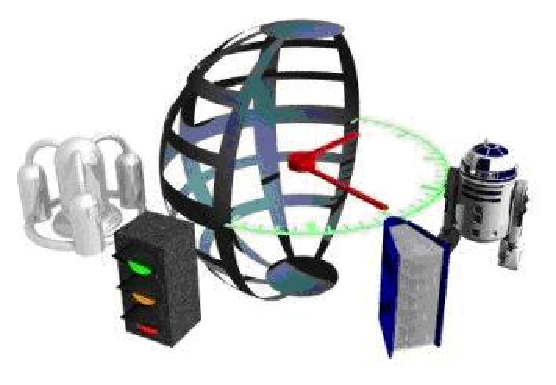
\includegraphics[width=0.5\textwidth]{image}
%    \caption{Numele figurii}
%    \label{fig:exemplu}
%\end{figure}
%
%
%Formula~(\ref{eq:example}) arată modul de calcul al lui $\Delta$:
%\begin{equation} \label{eq:example}
%    \Delta =\sum_{i=1}^N w_i (x_i - \bar{x})^2 .
%\end{equation}
%
%
%Algoritmul~\ref{alg:example} este un exemplu de descriere pseudo-cod a unui algoritm, preluat de la \href{http://en.wikibooks.org/wiki/LaTeX/Algorithms#Typesetting_using_the_algorithm2e_package}{http://en.wikibooks.org/wiki/LaTeX}. El utilizează pachetul \textit{algorithm2e}. Alternativ, puteți utiliza pachetele \textit{algorithmic} sau \textit{program}. 
%
%\begin{algorithm}
% \KwData{this text}
% \KwResult{how to write algorithm with \LaTeX2e }
% initialization\;
% \While{not at end of this document}{
%  read current\;
%  \eIf{understand}{
%   go to next section\;
%   current section becomes this one\;
%   }{
%   go back to the beginning of current section\;
%  }
% }
% \caption{How to write algorithms}
% \label{alg:example}
%\end{algorithm}

%\chapter{Implementation Details}
 \chapter{Detalii de implementare}
\label{cap:implementare}


\section{Structura codului sursa}

Codul folosit pentru obținerea sistemului \textit{thesistitle} este împărțit în 3 proiecte separate: 
\begin{itemize}
	\item \textbf {Tor activity monitor} ce constituie logica necesară obținerii listei de adrese IP blocate de sistem. 
	\item \textbf{SQLi SVM} scopul acestuia fiind obținerea modelului de SVM folosit pentru prevenirea atacurilor de SQL injection. 
	\item \textbf{\thesistitle} reprezentând sistemul propus și încorporează rezultatele obținute de celelalte două proiecte. 
\end{itemize}

\begin{figure}[h]
	\centering
	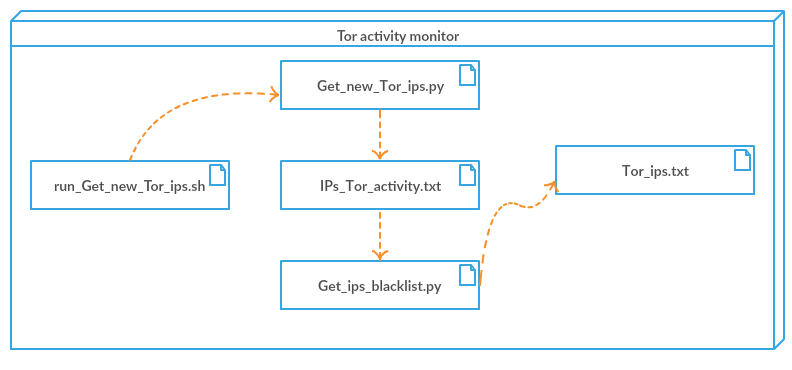
\includegraphics[width=0.8\textwidth]{tor_activity_monitor.png}
	\caption{Modulul pentru monitorizarea  activității rețelei Tor}
	\label{fig:tor_activity_monitor}
\end{figure}

Figura ~\ref{fig:tor_activity_monitor}  prezintă care sunt fișierele folosite pentru monitorizarea activității rețelei Tor și pentru obținerea listei cu adresele IP ce trebuie blocate de către sistem și relațiile dintre acestea. \\

\textbf{run\_Get\_new\_Tor\_ips.sh} este un fișier de bash ce are rolul de a rula Get\_new\_Tor\_ips.py. Fișierul este programat s a lanseze în execuție  Get\_new\_Tor\_ips.py  la ore fixe, acesta rulând încontinuu pe un sistem cu acces la internet neîntrerupt. Lansările în execuție au loc o data la 6 ore, respectiv la oră 12 am și pm și 6 am și pm. 

\textbf{Get\_new\_Tor\_ips.py}  are rolul de a documenta modificările de uptime din ultimele 6 ore ale nodurilor rețelei Tor. Datele sunt furnizate de pe pagina "Tor Network Status" \cite{tot_status} și pentru fiecare adresă IP prezentă în date, se verifică care este uptime-ul din ultimele 6 ore, informațiile acestea fiind stocate în  IPs\_Tor\_activity.txt.

\textbf{IPs\_Tor\_activity.txt}  are rolul de a stoca informațiile despre toate adresele IP utilizate de rețeaua tor din ultima luna. Acestea sunt salvate în liste, pentru fiecare adresă IP în parte o lista.  

\textbf{Get\_ips\_blacklist.py} are rolul de genera  fișierul  Tor\_ips.txt f olosit de către sistemul propus pentru blocarea adreselor IP. Acesta folosește datele din interiorul fișierului  IPs\_Tor\_activity.txt,  pentru a genera o lista cu toate adresele IP ce au un uptime total mai mare de 7 zile în ultimele 30 de zile. 

\textbf{Tor\_ips.txt}  reprezintă rezultatul proiectului. Acesta este alcătuit dintr-o lista formată din toate adresele IP ce vor fi blocate de sistemul propus în timpul rulării. 

\newpage

\begin{figure}[h]
	\centering
	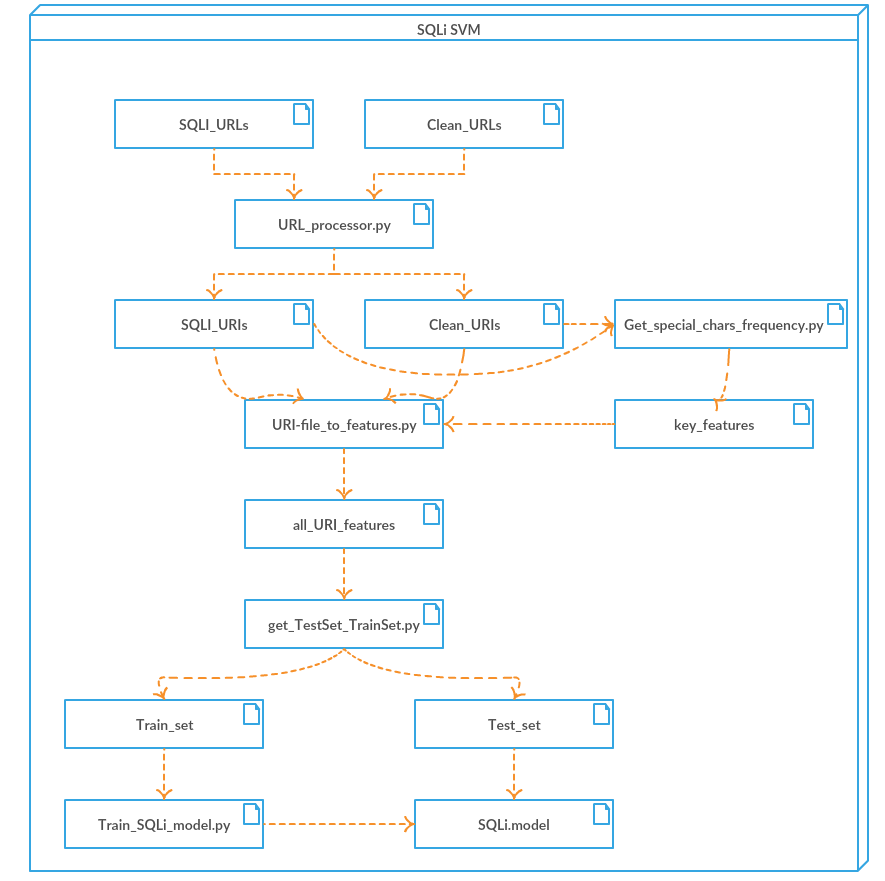
\includegraphics[width=0.8\textwidth]{sqli_svm.png}
	\caption{Modulul pentru prevenirea atacurilor SQL injection}
	\label{fig:sqli_svm}
\end{figure}
Figura ~\ref{fig:sqli_svm}  prezintă care sunt fișierele utilizate pentru procesarea datelor necesare în procesul de antrenare a modelului de SVM, până la obținerea modelului propriu-zis și care sunt relațiile dintre acestea. \\

\textbf{SQLI\_URLs}  reprezintă setul inițial de date "infected" folosite pentru identificarea atacurilor SQL injection. Acest set este constituit din URL-uri ce au fost identificate de un produs autorizat ca fiind tentative de SQL injection. 

\textbf{Clean\_URLs}  reprezintă setul inițial de date "clean" folosite pentru identificarea atacurilor SQL injection. Acest set este constituit din URL-uri ce au fost identificate de un produs autorizat ca fiind URL-uri curate. 

\textbf{URL\_processor.py}  primește ca input un fișier sau string și are rolul de a procesa URL-uri într-un format uniform(se elimină encodările) și specific pentru pașii următori. 

\textbf{SQLI\_URIs}  constituie nou lista rezultată din procesarea fișierului SQLI\_URLs de către URL\_processor.py.

\textbf{Clean\_URIs}  constituie noua lista rezultată din procesarea fișierului Clean\_URLs de către URL\_processor.py.

\textbf{Get\_secial\_chars\_frequency.py} are rolul de  a calcula frecvența de apariție a unor caractere speciale în cele două seturi de date și de a decide în funcție de frecvența lor de apariție, care din acestea sunt relevante în vederea alegerii trăsăturilor de clasificare. 

\textbf{key\_features} este  o listă alcătuită din toate cuvintele cheie a limbajului SQL, dar și din caracterele speciale utilizate în acesta și considerate ca fiind relevante în urma execuției scriptului  Get\_secial\_chars\_frequency.py.

\textbf{URI-file\_to\_features.py}  are rolul de a procesa cele două fișiere de date și pe baza trăsăturilor din  key\_features  să constituie un nou fișier ce conține pentru fiecare URL din cele două fișiere tipul acestuia și trăsăturile găsite în el, precum și frecvența lor.

\textbf{all\_URI\_features} este rezultatul rulării scriptului URI-file\_to\_features.py  și conține pentru fiecare URL din cele două fișiere de date, tipul acestuia și trăsăturile găsite în el, precum și frecvența lor, acestea fiind folosite pentru antrenarea și testarea modelului de SVM. 

\textbf{get\_TestSet\_TrainSet.py}  are rolul de a împarți datele prezente în  all\_URI\_features  în două seturi de proporție 70-30. Aceste două seturi fiind folosite pentru antrenarea și testarea modelului. 

\textbf{Train\_set} constituie 70\% din totalul de exemple acumulate pentru antrenarea modelului, doar acestea fiind de fapt folosite pentru antrenarea sa. 

\textbf{Test\_set} constituie 30\%  din exemplele acumulate, aceste date fiind folosite pentru testarea acurateții modelului după antrenare. 

\textbf{Train\_SQLi\_model.py} realizează obținerea modelului de SVM folosit de sistem pentru prevenirea atacurilor SQL injection. Pentru antrenare modelului este folosit setul de date din fișierul Test\_set și algoritmi puși la dispoziție de biblioteca open source libsvm  \cite{libsvm}.

\textbf{SQLi.model}  reprezintă rezultatul proiectului. Acesta este testat cu ajutorul setului de date din fișierul Test\_set și ulterior integrat în sistemul propus pentru a fi folosit pentru prevenirea atacurilor SQL injection. 

\newpage

\begin{figure}[h]
	\centering
	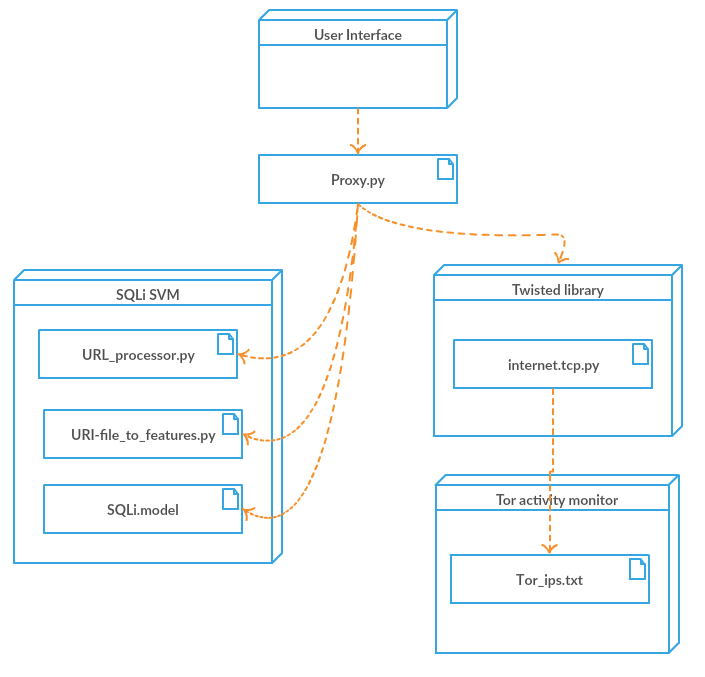
\includegraphics[width=0.8\textwidth]{source_code.png}
	\caption{ Interacțiunea dintre interfața grafică și celelalte module }
	\label{fig:source_code}
\end{figure}
Figura ~\ref{fig:source_code}  prezintă care sunt fișierele, specific fiecărui modul, care sunt accesate în mod direct de către interfață sau indirect de alte fișiere, în timpul rulării și relațiile dintre acestea. \\


\textbf{User Interface}  reprezintă întreaga componentă ce realizează interfața de utilizator cu toate fișierele necesare realizării ei incorporate în compoziția sa. Aceasta a fost realizată ca un proiect dezvoltat în .Net implicând multe fișiere cu scopul realizării elementelor grafice. Aceste elementu nu vor fi tratate în această secțiune. 

\textbf{Proxy.py}  reprezintă fișierul ce încorporează, respectiv leagă, tot codul ce constituie partea de "back end" a proiectului. În acest script de python se realizează instanțierea elementului de reverse proxy cu parametri de adrese IP și porturi aferente, precum și furnizarea metodelor de detecție componentei de reverse proxy. 

\textbf{Twisted library}  este o bibliotecă open source scrisă în Python, ce oferă suport pentru diferite protocoale(TCP, UDP, SSL/TLS). Biblioteca a fost folosită pentru partea de cod ce oferă implementarea unui reverse proxy. Mare parte din fișierele oferite de acesta bibliotecă au fost folosite fără a fi suprascrise sau a li se aduce modificări ulterioare, însă în vederea atingeri scopului propus, asupra unor fișiere sursă au fost aduse mici modificări(internet.tcp.py).

\textbf{internet.tcp.py} este scriptul din biblioteca twisted ce oferă suportul pentru protocolul TCP. Acest fișier a fost modificat pentru introducerea detecției împotriva utilizatorilor de Tor. Script-ul integrează lista realizată de proiectul "Tor activity monitor" pentru verificarea adresei utilizatorilor ce doresc să stabilească o conexiune TCP. 




\section{Algoritmi, metode si API-uri}

În acesta secțiune se urmărește descrierea codului sursă folosit la realizarea sistemului propus și explicarea amănunțită a codului/metodelor considerate mai relevante, precum și a principalelor api-uri utilizate în implementarea acestuia. Abordarea codului sursă se realizează conform sub-proiectelor prezentate în secțiunea anterioară(Tor activity monitor, AQLi SVM, Interfața utilizator). 

\subsection{Tor activity monitor}

Conform figurii ~\ref{fig:tor_activity_monitor},  acest proiect este realizat din 5 fișiere, acestea având o relație liniară între ele.

Fișierul ce începe ciclul de execuție,  run\_Get\_new\_Tor\_ips.sh, este un fișier de bash ce rulează în buclă infinită. Fișierul trebuie să ruleze pe un sistem ce este funcțional non-stop și cu acces nelimitat la internet. La ore fixe (12 am și pm și 6 am și pm), acesta lansează în execuție scriptul de python  Get\_new\_Tor\_ips.py.

Fișierul principal din acest proiect îl reprezintă  Get\_new\_Tor\_ips.py.  Acesta descărcă pagina "Tor Network Status" \cite{tot_status}  și procesează datele de pe acestea, introducând în fișierul IPs\_Tor\_ activity.txt  informații referitoare la adresele IP găsite pe pagină și uptime-ul lor din ultimele 6 ore. Procesarea adreselor IP și extragerea valorii lor de uptime se poate observa în următoarele două secvențe de cod. 

\lstset{language=python,frame=single, showstringspaces=false}
\begin{lstlisting}
time_up = row.findAll('td')[4].contents[0]
ip = row.findAll('td', attrs={'class':'iT'})[0].findAll('a',
 attrs={'class':'who'})[0].contents[0]


\end{lstlisting}

Pentru prelucrarea conținutului paginii, acesta a fost download-at în memoria programului, iar codul HTML rezultant a fost prelucrat cu ajutorul bibliotecii de python open source, BeautifulSoup. Codul de mai sus reprezintă extragerea valori de timp(uptime) și adresa IP căreia aceasta corespunde. Variabila "row" fiind un element din obiectul iterabil rezultat din inițializarea bibliotecii BeautifulSoup cu codul HTML al paginii. 

\lstset{language=python,frame=single, showstringspaces=false}
\begin{lstlisting}
days = time_up.split()[1]
if days == 'd':
    hours = 6
else:
    hours = int(time_up.split()[0])
    if hours > 6:
        hours = 6

\end{lstlisting}

În secvența de mai sus de cod, este identificata valoarea corectă de uptime din ultimele 6 ore. Pentru cazul în care valoare de uptime este sub formă de zile sau aceasta este mai mare de 6 ore, ea se setează pe 6 ore, întrucât nu ne interesează decât activitatea din ultimele 6 ore. 
\begin{lstlisting}
from bs4 import BeautifulSoup
from urllib.request import urlopen

pagesource = urlopen(page)
soup = BeautifulSoup(pagesource.read())
table = soup.findAll('table', attrs={'class': 'displayTable'})
\end{lstlisting}

Pentru procesarea  conținutului unei pagini web("Tor Network Status" \cite{tot_status}) s-au folosit bibliotecile de python, open source, urllib și BeautifulSoup \cite{btf_soup}.  Biblioteca urllib oferă funcții și clase ce pot fi folosite pentru deschiderea de URL-uri(urlopen). Funcția folosită în codul de mai sus primește ca parametru "page" adresa sub formă de string a paginii ce se dorește a fi citită. Biblioteca BeautifulSoup este o bibliotecă de python folosită pentru extragerea de date din fișiere de HTML sau XML. Acesta este inițializată cu un document HTML/XML și că rezultat oferă un obiect ce permite navigarea prin codul sursă asemeni unei structuri de date imbricate. Astfel, spre exemplu, pentru identificarea structurii corespunzătoare tabelei de adrese IP din codul sursă al paginii s-a folosit o singură linie de cod, în care s-au specificat numele și atributele specifice acesteia. 

Rezultatele rulării fișierului  Get\_new\_Tor\_ips.py sunt  actualizate în  IPs\_Tor\_activity.txt.  Acest fișier este de fapt un json în care se realizează dump la noul dicționar obținut de   Get\_new\_Tor\_ips.py.  Dicționarul este constituit din adresa IP ca și cheie și o listă .Structura acestor liste este realizată dintr-o serie de numere între 0 și 6 ce reprezintă timpul total de uptime corespunzător sfertului respectiv de zi. Dimensiunea acestei liste este fixată la 30(zile)*4(sferturi de zi), pe măsură ce un element nou este adăugat, primul element din lista fiind scos. 

Următorul pas este filtrarea tuturor adreselor IP ce au un uptime mai mare de 7 zile. Acest lucru este realizat de scriptul  Get\_ips\_blacklist.py, iar rezultatele sunt stocate în Tor\_ips.txt, o adresă IP pe linie. 

\subsection{SQLi SVM}
Desfășurarea proiectului începe de la cele două fișiere SQLi\_URLs si Clean\_URLs.  În aceste două fișiere se află URL-uri complete din categoria conformă cu numele fiecărui fișier. Aceste fișiere sunt procesate de scriptul  URI\_processor.py  care are rolul de a uniformiza datele în aceeași encodare. Următoarea bucată de cod prezintă secvența ce transformă valorile hexa dintr-un URI în caractere și modul în care erorile de encodare sunt tratate(sunt afișate pentru a fi tratate manual de către programator): 

\lstset{language=python,frame=single, showstringspaces=false}
\begin{lstlisting}
for index, sub_uri in enumerate(uri.split('%')):
    if sub_uri:
        if index == 0:
            new_uri = sub_uri
            continue
        try:
            hex_val = bytearray.fromhex(sub_uri[:2]).decode()
        except UnicodeDecodeError:
            print(uri + ' --- ' + sub_uri[:2])
            return ''
        new_uri += hex_val + sub_uri[2:]
\end{lstlisting}

Întrucât într-un URL caracterul '\%' nu poate să apăra decât dacă acesta este encodat('\%25'- valoarea pentru encodarea caracterului '\%'), identificarea tuturor caracterelor encodate a fost făcută prin identificarea tuturor caracterelor de tipul '\%' în URI. În cazul în care un astfel de caracter este găsit, se încearcă conversia următoarelor două caractere(așteptându-se, conform convenției, să fie cifre sau litere de la A la F), din valoarea în hexa corespunzătoare unui anumit caracter în caracterul în sine. 

  
În urma procesării datelor, rezultă cele două fișiere  SQLi\_URIs si Clean\_URIs,  acestea având același conținut ca cele anterioare însă în aceeași encodare. În urma obținerii acestor două fișiere, a fost realizată completarea listei de trăsături(lista inițială este constituită din toate cuvintele cheie a limbajului SQL) cu caracterele speciale întâlnite în acest limbaj. Scriptul  Get\_secial\_chars\_frequency.py  are rolul de a determina frecvența de apariție a fiecărui caracter special în cele două seturi de date, iar pe baza unei observații umane, a fost realizată determinarea caracterelor ce constituie trăsături rentabile. Următoarea bucată de cod este din scriptul Get\_secial\_chars\_frequency.py  și realizează numărarea URI-urilor(pentru comparare) din setul de date și frecvența caracterelor speciale("dict" este un dicționar cu cheile fiind caracterele speciale utilizate în limbaj): 
\lstset{language=python,frame=single, showstringspaces=false}
\begin{lstlisting}
with open(args.f, 'r') as fd:
    for lines in fd.readlines():
        lines_nr += 1
        line = lines.strip()
        for keys in dict:
            if keys in line:
                dict[keys] += 1
                
\end{lstlisting}

Pentru identificarea caracterelor relevante din limbajul SQL în comparație cu cele folosite într-un URL obișnuit, s-a ales numărarea frecvenței de apariție a acestora în URL-uri normale, dar și în URL-uri ce conțin atacuri de SQL injection. Numărarea se face alternativ, rezultatele fiind furnizate că două seturi de date separate, bucata anterioară de cod reprezentând procesul doar pentru una dintre cele două categorii. Dicționarul referit în cod este alcătuit dintr-un dicționar ce are că și chei valoarea caracterelor speciale căutate, iar ca valoare, acestea sunt inițializate pe zero pentru a fi incrementate o data cu numărul de apariții ale caracterelor căutate. Pentru uniformizarea setului de date, întrucât distribuția acestor caractere nu este tot timpul uniformă, se ține cont și de numărul de linii(pe fiecare linie se află un URI distinct) în care au fost identificate frecvențele lor de apariție. 

După determinarea caracterelor relevante, acestea au fost completate manual în fișierul key\_features, fișier ce însumează toate trăsăturile ce sunt folosite în antrenarea modelului(fiecare linie conține o trăsătură, numărul liniei fiind și indicele de referință a trăsăturii). 

Pentru obținerea datelor într-un format ce poate fi procesat de biblioteca libsvm \cite{libsvm} a fost necesară transformarea acestora într-un anumit format: 

\begin{lstlisting}
+1 23:1 37:4 103:2
-1 54:1 77:1
\end{lstlisting}

Conversia URI-urilor în formatul de mai sus este realizată de scriptul  URI-file\_to\_features.py.  Formatul de mai sus este reprezentarea fiecărui URL în funcție de tipul acestuia și indicele trăsăturii găsite în interiorul sau precum și frecvența de apariție a acestora(tip trăsătură : trăsătură : frecvență). Următoarele bucăți de cod sunt extrasă din fișieru l URI-file\_to\_features.py  și realizează conversia unui URI în echivalentul sau în trăsături: 

\begin{lstlisting}
if keys in uri:
 if keywords_list.index(keys) > 184:
  keywords[keys] = uri.count(keys)
  if not uri.count(keys) == 0:
    ok = True
\end{lstlisting}

În lista cu trăsături, primele 184 de poziții corespund cuvintelor cheie ale limbajului SQL, următoarele 8 poziții aparținând trăsăturilor de tipul caracter special(determinate la pasul anterior de script-ul "Get\_special\_chars\_frequency.py"). În cazul în care o astfel de trăsătură este găsită într-un URI, pur și simplu se găsește numărul total de apariții a caracterului respectiv în URI. 


\begin{lstlisting}
sub_uri = uri.split(keys)
for index, ele in enumerate(sub_uri):
  if index + 1 < len(sub_uri):
    if ele and sub_uri[index + 1] and not ele[-1].isalpha()
     and not sub_uri[index+1][0].isalpha():
      keywords_aux[keys] += 1
  elif not ele and sub_uri[index - 1]:
      keywords_aux[keys] += 1
\end{lstlisting}

Pentru trăsăturile de pe primele 184 de poziții, adică cuvintele cheie ale limbajului SQL, s-a abordat o logică mai complexă de procesare. O data ce un cuvânt este găsit într-un URI, pentru fiecare apariție a acestui cuvânt se verifică ca primul caracter anterior cuvântului și primul următor cuvântului să nu fie literă, astfel eliminându-se cazurile în care unele cuvinte sunt incluse în altele(ex:  \textbf{all} și de\textbf{all}ocate).

În urma procesării fișierelor de date, rezultă un fișier (all\_URI\_features)  ce însumează toate datele utilizate în antrenarea modelului(exemple atât pozitive cât și negative), însă sub formă prezentată anterior(tip trăsătură :  trăsătură : frecvență). Acest fișier este împărțit în două fișiere cu proporția  de 70\% pentru Train\_set și 30\% Tes\_set de scriptul get\_Trainset\_Testset.py.  cu scopul de a obține un grup de date atât pentru antrenarea modelului cât și pentru testarea ulterioară a acestuia. 

Pentru antrenarea modelului, s-a folosit biblioteca open sourece libsvm. Această bibliotecă furnizează fișierele necesare antrenării modelului de svm și de prezicere a unui rezultat pe un model existent. Apelul către executabilul "svm-train.exe" se face prin intermediul scriptului de python  Train\_SQLi\_model.py.
Executabilul de windows furnizat de biblioteca libsvm poate fi apelat conform exemplului următor: 

\begin{lstlisting} 
svm-train.exe [options] training_set_file [model_file]
\end{lstlisting}

\subsection{Interfață utilizator}

 Componenta de interfață reprezintă atât proiectul în .net în care a fost realizată interfață sistemului, dar și fișierele/script-urile ce au rolul de a interconecta rezultatele celor două proiecte anterioare cu acesta. 

Scriptul Proxy.py încapsulează toate elementele, din partea de back end, a proiectului propus. Acesta de asemenea furnizează ca output într-un format specific(format ce este cunoscut și interpretat de interfața grafică) toate evenimentele ce apar în timpiul rulării sistemului. În acest script se realizează instanțierea elementului de reverse proxy cu parametri de adrese IP și porturi aferente, precum și furnizarea metodelor de detecție componenței de reverse proxy. Inițializarea elementului de reverse proxy se realizează cu ajutorul codului oferit de biblioteca twisted. Acest cod este prezentat în "Anexa A" a acestei lucrări. 

În următoarele imagini sunt prezentate posibilele pagini ale interfeței utilizator precum și o scurtă descriere ce ilustrează funcționalitățile oferite de paginile respective pentru utilizator. 
\newpage]
 
\begin{figure}[h]
	\centering
	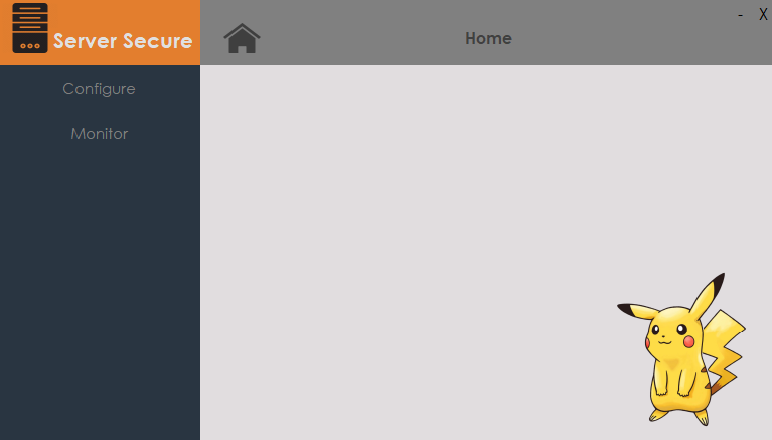
\includegraphics[width=0.6\textwidth]{ui_home.png}
	\caption{Meniul "Home" in interfata grafica}
	\label{fig:ui_home}
\end{figure}
Figura ~\ref{fig:ui_home}  prezintă design-ul paginii de "Home" din interfața grafică pusă la dispoziție utilizatorilor sistemului. Acesta pagină este afișată la lansarea în execuție a aplicație, dar poate fi accesata de către utilizator și prin apăsarea butonului în formă de "căsuță" din dreapta logoului aplicației. \\

\begin{figure}[h]
	\centering
	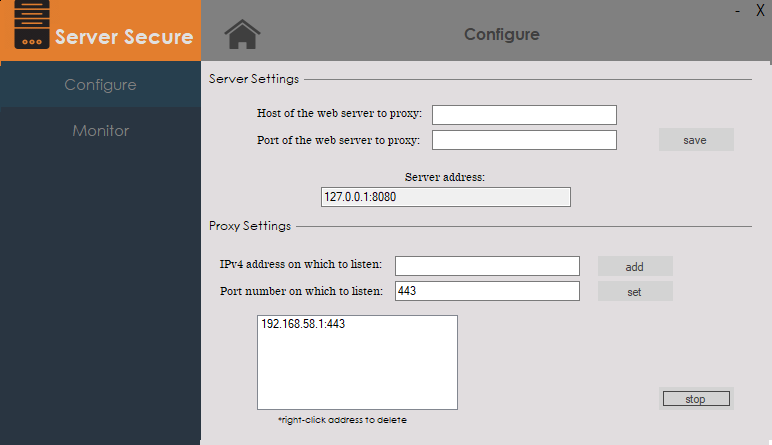
\includegraphics[width=0.7\textwidth]{ui_configure.png}
	\caption{Meniul "Configure" in interfața grafica}
	\label{fig:ui_configure}
\end{figure}
Figura ~\ref{fig:ui_configure}  prezintă design-ul paginii de "Configure" din interfața grafică, în care utilizatorul sistemului poate să seteze interfețele și porturile care vor fi tratate în timpul rulării. Partea superioară a meniului reprezintă setările aferente părții de server, precum sugerează și eticheta din stânga sus "Server Settings". În partea inferioară se pot seta detaliile interfețelor ce se pot conecta la server-ul setat mai sus (aceste interfețe pot fi multiple).  \\

\begin{figure}[h]
	\centering
	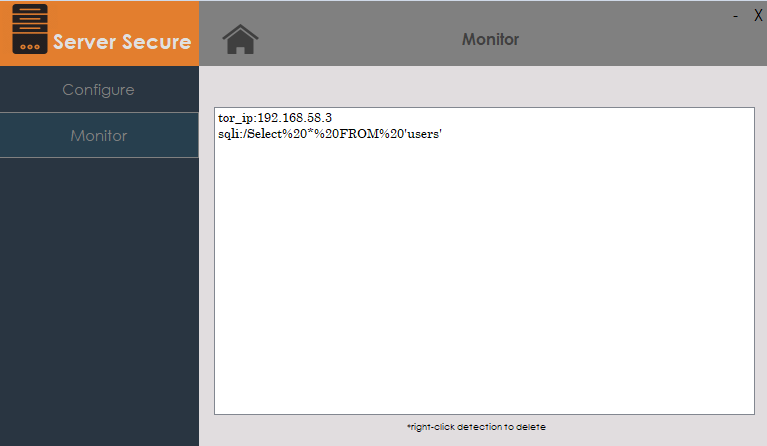
\includegraphics[width=0.8\textwidth]{ui_monitor.png}
	\caption{Meniul "Monitor" in interfața grafica}
	\label{fig:ui_monitor}
\end{figure}
Figura ~\ref{fig:ui_monitor}  prezintă design-ul paginii de "Monitor" din interfața grafică, în care utilizatorul poate să urmărească activitatea sistemului în timpul rulării. În această fereastră apar evenimentele apărute în timpul rulării aplicației, evenimente ce sunt sub formă de detecții. \\

\begin{figure}[h]
	\centering
	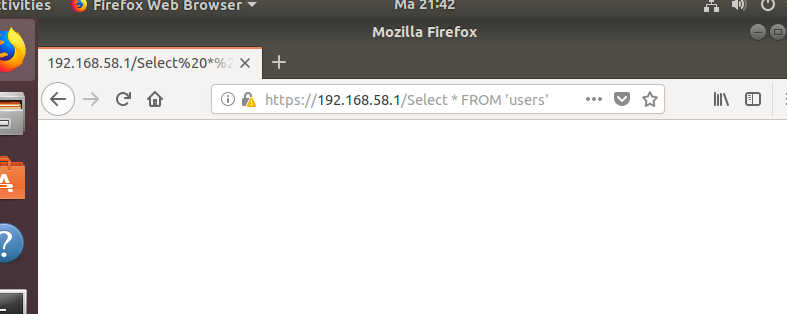
\includegraphics[width=0.9\textwidth]{sqli_respons.png}
	\caption{Raspunsul pentru SQL injection URL}
	\label{fig:sqli_respons}
\end{figure}

Figura ~\ref{fig:sqli_respons}  prezintă cum arată răspunsul primit de la server de către un utilizator după trimiterea unui request către server, cu intenția de a realiza un atac de tipul SQL injection. Utilizatorului i se returnează o pagină goală. \\
\newpage

\begin{figure}[h]
	\centering
	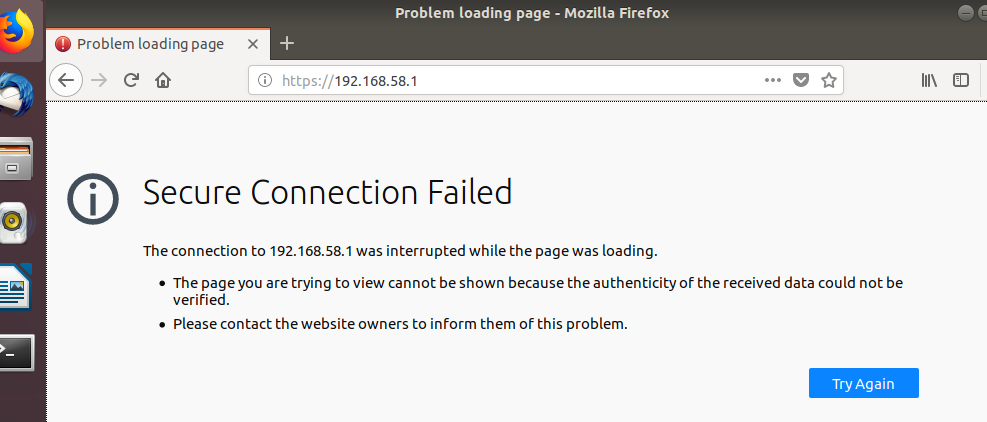
\includegraphics[width=0.8\textwidth]{tor_respons.png}
	\caption{Principalele module ale sistemului propus}
	\label{fig:tor_respons}
\end{figure}
Figura ~\ref{fig:tor_respons}  prezintă cum arată răspunsul primit de la server de către un utilizator al rețelei Tor ce intenționează să se conecteze la acesta. Acestor utilizatori li se refuză conexiunea.  \\


%
%
%Conține detalii de implementare: 
%\begin{itemize}
%  \item organizarea codului sursă, organizarea logică a codului (module, ierarhii de clase)
%  \item descrierea claselor, funcțiilor, API-urilor importante ale aplicației
%  \item descrierea la nivel de implementare a algoritmilor principali
%  \item descrierea părților mai dificile
%  \item alte detalii de implementare relevante, specifice fiecărei aplicații
%\end{itemize}
%
%Descrierea implementării trebuie să reflecte modul în care ea corespunde (se mapează) design-ului. 
%
%Nu se vor da detalii irelevante. Descrierea codului trebuie gândită ca un ghid de parcurgere a codului sursă de către cineva care vrea să continue proiectul vostru. 
%
%Exemplu de cod:
%\lstset{language=C,frame=single, showstringspaces=false}
%\begin{lstlisting}
%# include <stdio.h>
%  
%int main (int argc, char **argv)
%{
%  int i;
%    
%  for (i=0; i<argc; i++)
%    printf("argv[%d] = %s\n", i, argv[i]);
%    
%  return 0;
%}
%\end{lstlisting}

%\chapter{Tests and Results}
 \chapter{Teste și rezultate experimentale}
\label{cap:rezultate}

%Ponderea acestui capitol relativ la întreaga lucrare este de 5-10\%.
%
%Aici sunt prezentate metodele de validare a soluțiilor/sistemului descris în capitolele anterioare, scenariile de testare a corectitudinii funcționale, a utilizabilității, performanței etc.   
%
%Rezultatele testelor experimentale necesită, în general interpretări (dacă rezultatele obținute corespund așteptărilor, intuițiilor cititorului, de ce apar variații/excepții etc.) și comparații cu rezultatele altor metode similare. 
%
%Sistemele de testare și testele propriu-zise trebuie descrise detaliat astfel încât să poată fi reproduse și de alții care poate vor să-și compare soluțiile lor cu a voastră (eventual, codul testelor poate fi pus în anexe). Dacă se poate alegeți pentru evaluarea sistemului vostru benchmark-uri (pachete de testare) dedicate, astfel încât comparația cu alte sisteme să poată fi făcută mai ușor. În plus, astfel de teste sunt mult mai complete și mai realiste decât cele dezvoltate de voi. Oricum, încercați ca testele efectuate să nu fie triviale, ci să acopere scenarii cât mai reale, mai complexe și mai relevante ale funcționării sistemului vostru. 

%\section{Functional Tests}
 \section{Teste de funcționalitate}
 
În testarea sistemului s-a pus accentul pe testare celor două funcționalități de protecție împotrivă atacurilor de SQL injection și a utilizatorilor de Tor. 

Pentru testarea modelului folosit în prevenirea atacurilor de SQL injection s-a folosit setul de date de test specificat și în capitolul ~\ref{cap:implementare}. Acest set a fost obținut din setul inițial de date de antrenare, acesta fiind împărțit în 2 seturi separate cu proporția de 70\%(set antrenare) și respectiv 30\%(set testare). 
 
\begin{center}
	\begin{tabular}{||c c c c||} 
		\hline
		Tip set de testare  & Preziceri corecte & Dimensiune set & Acuratete(\%) \\ [0.5ex] 
		\hline\hline
		Clean \& infected & 187596 & 189278 & 99.11 \\ 
		\hline
		Clean & 5466 & 6258 & 87.34 \\
		\hline
		Infected & 182130 & 193020 & 99.51 \\
		\hline
	\end{tabular}
\end{center}

Pe baza tabelului de mai sus se pot observa diferențe majore de performanta între detecția pe setul "Clean" și pe "Infected". Aceste diferențe, respectiv scăderi de performanță în cazul setului Clean, se datorează dimensiunii mult mai mici a setului de Clean folosit și în antrenarea modelului. 

Pentru testarea eficienței sistemului de blocare a adreselor IP ale rețelei Tor, s-a realizat o referință între datele colectate de modulul de monitorizare a activității rețelei Tor. 

În prima diagrama este prezentată diferența procentuală dintre adresele IP cu un uptime mai mare de 7 zile în ultima lună și cele cu un uptime mai mic. În cea de a doua diagramă este evidențiată diferența dintre uptime-ul total ale acestor adrese IP din ultima lună. Printr-o analiză simplă în paralel a datelor din cele două diagrame, se poate observa că deși doar 20.31\% din IP-urile folosite de rețeaua Tor sunt blocate, din timpul total de uptime din ultima lună, 75.6\% aparține acestor adrese IP .

\begin{figure}
	\centering
	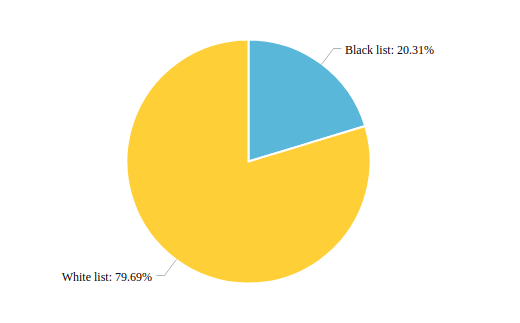
\includegraphics[width=0.7\textwidth]{test_case_1.png}
	\caption{ Raportul dintre numărul IP-urilor de pe Blacklist și Whitelist dintr-o lună }
	\label{fig:test_1}
\end{figure}

\begin{figure}
	\centering
	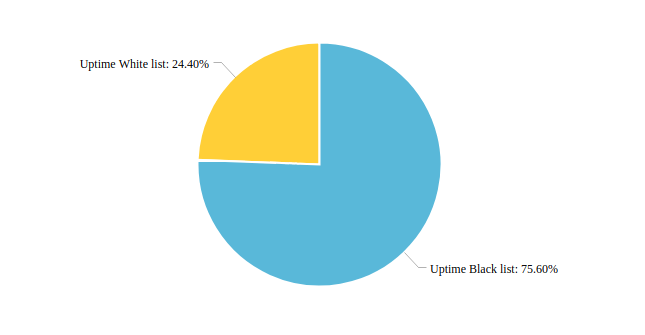
\includegraphics[width=0.7\textwidth]{test_case_2.png}
	\caption{ Raportul dintre uptime-ul IP-urile de pe Blacklist și Whitelist din aceeași lună }
	\label{fig:test_2}
\end{figure}


\newpage
%\section{Performance Tests}
 \section{Teste de performanță}

Sistemul propus a fost testat pe două configurații diferite pentru PC-ul gazdă: Intel Core i7-6600U CPU cu 4 nuclee și o frecvență de 2.6 GHz, cu 16 GB RAM DDR4 și i7-4790k CPU cu 4 nuclee și o frecvență maximă de 4.0 GHz, cu 16 GB RAM DDR4. Ambele sisteme furnizând mult mai multe resurse decât cele necesare unei funcționari optime. În cea ce privește resursele minime necesare, acestea trebuie să fie cele necesare rulării unui sistem de operare Windows 10: un procesor cu o frecvență mai mare de 1.0 GHz și o memorie mai mare sau egală cu 2 GB de RAM. În cea ce privește capacitățile sistemului de a suporta conexiuni exterioare, acesta nu a fost testat decât manual, prin intermediul unor mașini virtuale. 

%User Manual
%\chapter{User Manual}
 \chapter{Manual utilizator}

\label{cap:user-manual}
%
%Descrie pașii de instalare și rulare a aplicației. Dacă dezvoltarea aplicației s-a bazat sau a presupus instalarea și configurarea unei infrastructuri (complexe), descrieți detaliat pașii pe care i-ați urmat (referințele utilizate) și mai ales abaterile voite sau necesare de la documenațiile referite. Încercați ca cineva care vă continuă tema să nu mai fie nevoit să mai piardă timp inutil cu pregătirea mediului de lucru și să poată trece cât mai repede la abordarea temei proptriu-zise a proiectului. 
%
%Indincați, de asemenea, explicit versiunile aplicațiilor, bibliotecilor folosite și salvați o copie a acestora pe CD-ul atașat lucrării. E posibil ca aplicația voastră să nu mai funcționeze la fel pe alte versiuni și e bine de știut acest lucru și,  în același timp, e bine ca mediul descris de voi să poată fi reprodus ulterior. 
%
%Se întinde pe aproximativ 2-3 pagini. 

\section{Instalarea proiectului}

Pentru instalarea sistemului, atât timp cât toate dependințele acestuia sunt împlinite, utilizatorul nu mai trebuie să facă nimic. Toate fișierele necesare sistemului au fost împachetate în modulul principal, singurul pas ce poate fi executat de utilizator este crearea unui shortcut către executabilul ce lansează în execuție sistemul. 
\section{Utilizare}

După deschiderea aplicației, utilizatorul este întâmpinat de meniul de Home al acesteia. În următoarea fereastră se poate observa designul acestuia:  

\begin{figure}[h]
	\centering
	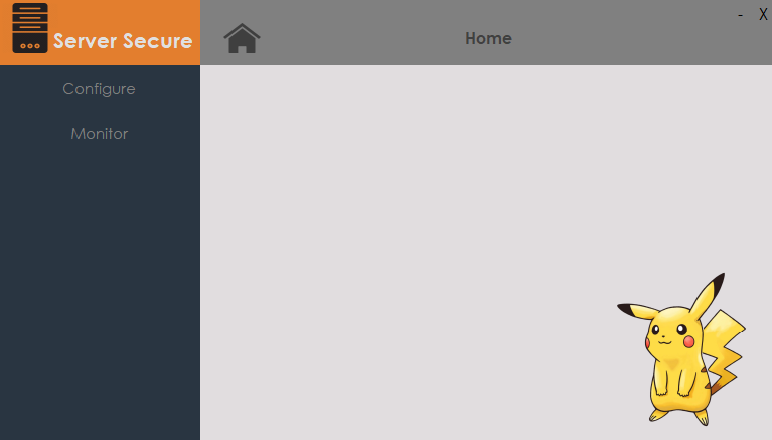
\includegraphics[width=0.6\textwidth]{ui_home.png}
	\caption{ Meniul "Home" în interfața grafică }
	\label{fig:ui_home}
\end{figure}

În partea superioară a ferestrei se află în permanență numele ferestrei curente(în cazul de față fereastra Home). În meniul prezent în stânga ferestrei sunt situate celelate două ferestre disponibile utilizatorului: Configure și Monitor. Utilizatorul poate să navighze între aceste ferestre dând un click pe numele ferestrelor, respectiv pe pictograma în formă de căsuță pentru meniul Home.  \\

\begin{figure}[h]
	\centering
	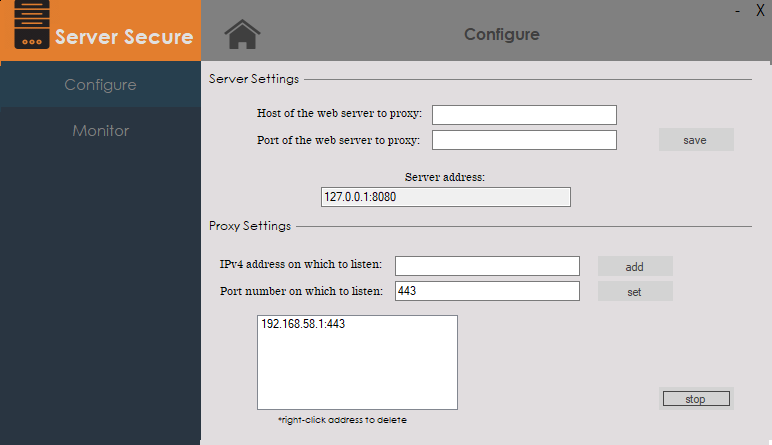
\includegraphics[width=0.7\textwidth]{ui_configure.png}
	\caption{ Meniul "Configure" în interfața grafică }
	\label{fig:ui_configure}
\end{figure}

În fereasra Configure, utilizatorul poate să seteze parametrii de rulare a sistemului. Acestuia i se prezintă două rubrici: Server Settings și Proxy Settings. În partea de Server Settings, utilizatorul setează datele server-ului: adresa IP a acestuia și portul aferent pe care acesta acceptă conexiunui. Salavarea sau suprascrierea acestor date se realizează prin apăsarea butonului "save" din rubrica respectivă. În partea de Proxy Settings, utilizatorul poate să introducă mai multe adrese IP și un port, pe care sistemul să accepte conexiuni și să le redirectioneze către server. După setarea parametrilor de mai sus, sistemul se poate porni/opri prin apăsarea butonului din dreapta jos(cu textul "start"/"stop" după caz). 
\newpage
\begin{figure}[h]
	\centering
	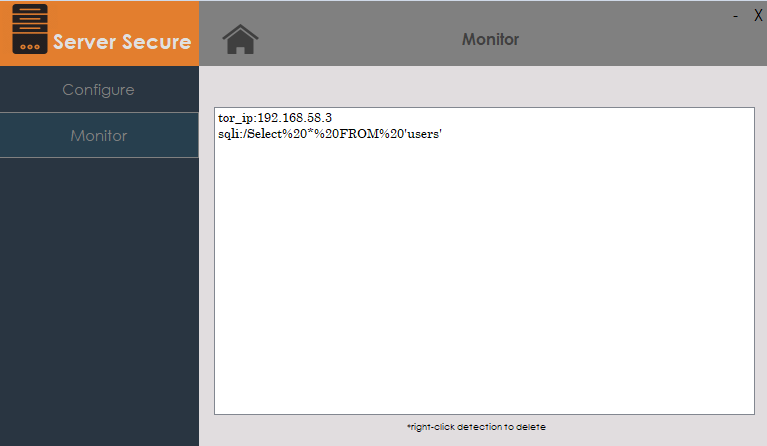
\includegraphics[width=0.8\textwidth]{ui_monitor.png}
	\caption{ Meniul "Monitor" în interfața grafică }
	\label{fig:ui_monitor}
\end{figure}

În fereastra de Monitor, utilizatorul poate să urmărească activitatea sistemului. În cazul în care sistemul detectează un eveniment, acesta este afișat în interfața grafică în această fereastre(conform exemplului din imagine). Dacă utilizatorul dorește ștergerea evenimentelor antrioare, aceasta se poate realiza prin click dreapta pe eveniment. 

%\chapter{Conclusions}
 \chapter{Conluzii}
\label{cap:concluzii}
\section{Privire de ansamblu asupra sistemului}

In urma eforturilor depuse, s-a realizat un sistem de prevenirea a intruziunilor care indeplineste aproape in intregime obiectivele initial propuse, mici inconveniente fiind la partea de performanta in detectie a sistemului. In cea ce priveste performanta sistemului, in cazul detectiei atacurilor de SQL injection(precum se poate vedea si in capitolul 7) procentul de fals pozitiv este mult mai mare decat se intentiona initial(12.66\% in loc de 3-4\%), insa acest lucru datorandu-se in principal setului mic de date de antrenare avute la dispozitie.

Prin implementarea detectiei atacurilor SQL injection folosind tehnici de machine learning, s-au dobandit cunostinte valoroase si experienta ce pot fi folosite in viitoare proiecte. Intrucat in practica, abordarea acestui subiect a reprezentat un lucru nou, o mare parte din timpul investit in dezvoltarea sistemului a reprezentat documentarea si acumularea de noi cunostinte si experienta pentru rezolvarea unor probleme cu tehnici de machine learning.

\section{Dezvoltari ulterioare}

Datorita unei abordari modulare a dezvoltarii sistemului, acestuia ii pot fi adaugate cu usurinta noi functionalitati.
 
Sistemul prezinta doua posibilitati majore de dezvoltari ulterioare, acestea fiind aferente celor doua tipuri de protectie implementata. In cazul protectiei impotriva adreselor IP malitioase, lista folosita momentan si poate extinde cu usurinta sau prin mici modificari in cod se pot adauga noi liste.

Protectia bazata pe detectia unui anumit continut in URL poate fi cu usurinta extinsa, prin adaugarea de noi model de machine learning sau noi logici de detectie, ambele cazuri necesitand mici modificari in codul sursa.

%Cuprinde:
%
%\begin{itemize}
% \item un rezumat al contribuțiilor aduse: ce s-a realizat, relativ la ce s-a propus, în ce constă experiența acumulată, care au fost punctele dificile atinse și rezolvată, recomandări pentru alții care abordează tema, la ce este bun ce s-a obținut etc.
% 
% \item a analiză critică a rezultatelor obținute: avantaje, dezavantaje, limitări
% 
% \item o descriere a posibilelor dezvoltări și îmbunătățiri ulterioare
%\end{itemize}
%
%Poate fi organizat pe secțiuni, dacă se dorește.
%
%Se întinde pe aproximativ 1-2 pagini. 








%\addcontentsline {toc}{chapter}{Bibliography}
\bibliographystyle{IEEEtran}
\bibliography{thesis}%same file name as for .bib

\appendix

\chapter{Codul sursa(principalele fisiere)}
\section{Reverse proxy}

\begin{lstlisting}
class BadURL(Resource):
  def render(self, request):
    return ""

class HTTPSReverseProxyResource(proxy.ReverseProxyResource, 
                                object):
  def getChild(self, path, request):
    global m

    features = uri_convertor.uri_to_features(request.uri)
    x0, max_idx = gen_svm_nodearray(features)
    label = libsvm.svm_predict(m, x0)

    if int(label) == 1:
    print('blocked-->sqli:' + request.uri)
    return BadURL()

    child = super(HTTPSReverseProxyResource, self).
                              getChild(path, request)
    return HTTPSReverseProxyResource(child.host, 
                  child.port, child.path, child.reactor)

def main(args):

  ap = argparse.ArgumentParser()
  ap.add_argument('-c', type=str, default='./server.crt')
  ap.add_argument('-k', type=str, default='./server.key')
  ap.add_argument('-m', type=str, default='./sqli.model')
  ap.add_argument('--server-ip', type=str,default='localhost')
  ap.add_argument('--server-port', type=int, default=8080)
  ap.add_argument('--listen-ip', type=str, default
  		=['192.168.58.1', 'localhost'])
  ap.add_argument('--listen-port', type=int, default=443)
  ns = ap.parse_args(args[1:])

  global m
  m = svm_load_model(ns.m)

  if type(ns.listen_ip) == str:
    ns.listen_ip = ast.literal_eval(ns.listen_ip)
  myProxy = HTTPSReverseProxyResource(ns.server_ip, 
  			ns.server_port, '')
  site = server.Site(myProxy)
  if ns.c:
    with open(ns.c, 'rb') as fp:
    ssl_cert = fp.read()
    if ns.k:
      with open(ns.k, 'rb') as fp:
      ssl_key = fp.read()
      certificate = ssl.PrivateCertificate.load(ssl_cert,
      	 ssl.KeyPair.load(ssl_key, crypto.FILETYPE_PEM),
      	 crypto.FILETYPE_PEM)
    else:
      certificate = ssl.PrivateCertificate.loadPEM(ssl_cert)
      for ele in ns.listen_ip:
        try:
          reactor.listenSSL(ns.listen_port, site, 
          	certificate.options(), interface=ele)
        except error.CannotListenError:
          print('Error: ' + ele + 
          ' not a valid interface in this context')
          exit(0)
        except Exception as e:
          print('Error: ' + e.message)
          exit(0)
  else:
    for ele in ns.listen_ip:
      try:
        reactor.listenTCP(ns.listen_port, site, interface=ele)
      except error.CannotListenError:
        print('Error: ' + ele + 
       		' not a valid interface in this context')
        exit(0)
      except Exception as e:
        print('Error: ' + e.message)
        exit(0)
  reactor.run()

if __name__ == '__main__':
  main(sys.argv)
\end{lstlisting}

\section{Convertor de URI in trasaturi pentru modelul SVM}
\begin{lstlisting}

def convert_uri(uri):
  new_uri = ''

    for index, sub_uri in enumerate(uri.split('%')):
      if sub_uri:
        if index == 0:
          new_uri = sub_uri
          continue
      try:
        hex_val = bytearray.fromhex(sub_uri[:2]).decode()
      except UnicodeDecodeError:
        hex_val = ''
      except ValueError:
        print(uri + ' --- ' + sub_uri[:2])
        return ''
      except Exception as e:
        print(str(e))
        print(uri + '---' + sub_uri[:2])
        exit(0)

      new_uri += hex_val + sub_uri[2:]
    new_uri = new_uri.upper()

return new_uri


def uri_to_features(uri):

  global keywords
  global keywords_list

  uri = convert_uri(uri)

  keywords_aux = keywords.copy()
  ok = False

  try:
    for keys in keywords_aux:
      if keys in uri:
        if keywords_list.index(keys) > 184:
        keywords_aux[keys] = uri.count(keys)
          if not uri.count(keys) == 0:
            ok = True
        else:
          sub_uri = uri.split(keys)
          for index, ele in enumerate(sub_uri):
            if index + 1 < len(sub_uri):
              if ele and sub_uri[index + 1]:
                if not ele[-1].isalpha() and not
                	 sub_uri[index+1][0].isalpha():
                  keywords_aux[keys] += 1
                  ok = True
            else:
              if not ele and sub_uri[index - 1]:
                keywords_aux[keys] += 1
                ok = True
  except:
    ok = False

  if ok:
    features = {}
    for keys in keywords_list:
      if not keywords_aux[keys] == 0:
        features[keywords_list.index(keys)+1] = 
        			keywords_aux[keys]
    keywords_aux.clear()
    return features
  else:
    keywords_aux.clear()
    return {}


def main(argv):

  parser = argparse.ArgumentParser()
  parser.add_argument('-u', type=str, help='uri to convert')

  args = parser.parse_args(argv[1:])

  if not args.u:
    print('No given string(uri)')
    exit(0)

  uri = convert_uri(args.u)

  print(uri)


if __name__ == '__main__':
  main(sys.argv)
\end{lstlisting}
\section{Monitorizarea adreselor IP ale retelei Tor}
\begin{lstlisting}
import re
import os
import json
from urllib.request import urlopen
from bs4 import BeautifulSoup

regex = re.compile(
  r'^(?:http|ftp)s?://' # http:// or https://
  r'(?:(?:[A-Z0-9](?:[A-Z0-9-]{0,61}[A-Z0-9])?\.)
  	+(?:[A-Z]{2,6}\.?|[A-Z0-9-]{2,}\.?)|' #domain...
  r'localhost|' #localhost...
  r'\d{1,3}\.\d{1,3}\.\d{1,3}\.\d{1,3})' # ...or ip
  r'(?::\d+)?' # optional port
  r'(?:/?|[/?]\S+)$', re.IGNORECASE)

all_ip = {}

def isValidUrl(url):
  if regex.match(url) is not None:
    return True
  return False
  

def sort_ip_list(ip_list):

  from IPy import IP
  ipl = [(IP(ip).int(), ip for ip in ip_list]
  ipl.sort()
  return [ip[1] for ip in ipl]

def init_dictionary():

  all_ip['0.0.0.0'] = []

def pars():

  global all_ip
  if not os.path.isfile('/home/avid/work/scenarii/bitbucket
  		/craw_tor/ips_tor_activity'):
    init_dictionary()
  else:
  with open('/home/avid/work/scenarii/bitbucket/craw_tor
  	     /ips_tor_activity', 'r', encoding='utf8') as fd:
    all_ip = json.load(fd)

  page = 'https://torstatus.blutmagie.de
  		/index.php?SR=Uptime&SO=Desc'

  pagesource = urlopen(page)
  s = pagesource.read()
  soup = BeautifulSoup(s)
  table = soup.findAll('table',attrs={'class':'displayTable'})
  rows = table[0].findAll('tr', attrs={'class': 'r'})

  current_tor_ips = {}

  for row in rows:

    try:
      time_up = row.findAll('td')[4].contents[0]
      ip = row.findAll('td', attrs={'class': 'iT'})[0].findAll
      ('a', attrs={'class': 'who'})[0].contents[0]

      days = time_up.split()[1]
      if days == 'd':
        hours = 6
      else:
        hours = int(time_up.split()[0])
        if hours > 6:
          hours = 6
    except:
      continue
    current_tor_ips[ip] = hours

  for ips in all_ip:
    if ips == '0.0.0.0':
      continue
    if ips not in current_tor_ips:
      all_ip[ips].append(0)
      continue
    all_ip[ips].append(current_tor_ips[ips])
    del current_tor_ips[ips]

  for ips in current_tor_ips:
    all_ip[ips] = all_ip['0.0.0.0'].copy()
    all_ip[ips].append(current_tor_ips[ips])

  all_ip['0.0.0.0'].append(0)

  with open('/home/avid/work/scenarii/bitbucket/craw_tor/
  	ips_tor_activity', 'w', encoding='utf8') as fd:
    json.dump(all_ip, fd)

pars()
\end{lstlisting}

\end{document}
